\documentclass[]{llncs}
\pagestyle{plain}

\let\proof\relax
\let\endproof\relax

\usepackage{amsmath}
\usepackage{amssymb}
\usepackage{amsthm}
\usepackage{amsfonts}
\usepackage{tikz}
\usepackage{todonotes}
\usepackage{xspace}
\usepackage{csquotes}
\usepackage{xfrac} % slanted fraction \sfrac

\usepackage{cleveref}
% cleveref config
\crefname{lemma}{lemma}{lemmas}
\Crefname{lemma}{Lemma}{Lemmas}
\crefname{theorem}{theorem}{theorems}
\Crefname{theorem}{Theorem}{Theorems}
\crefname{algocfline}{line}{lines}
\Crefname{algocfline}{Line}{Lines}

\usepackage{url}

\usepackage[linesnumbered,noend,noline]{algorithm2e}

\usepackage{changepage} % adjustwidth
\usepackage{comment}

\usepackage[utf8]{inputenc}
\usepackage[english]{babel}


\newif\iffull
\fulltrue


% Algorithm settings
\SetAlFnt{\small}
\SetKwInput{KwInput}{In}
\SetKwInput{KwOutput}{Out}
\SetKwProg{Fn}{}{:}{}
\SetInd{0.5em}{0.5em}
\SetKwFor{For}{for}{:}{}
\SetKwSwitch{Switch}{Case}{Other}{switch}{:}{case}{otherwise}{}


%\renewcommand{\vec}[1]{\boldsymbol{#1}}
%\let\vec\mathbf

% theorem environments
\newtheorem{protocol}{Protocol}%[section]
\newtheorem{construction}{Construction}%[section]

\newenvironment{subproof}[1][\proofname]{%
  \renewcommand{\qedsymbol}{$\blacksquare$}%
  \begin{proof}[#1]%
}{%
  \end{proof}%
}

\title{%
  \ourschemelong: Stacked Garbling\\
  with $O(b \log b)$ Computation
}
% \subtitle{Non-interactive Branching with $O(b \log b)$ Computation}
\titlerunning{\ourschemelong}
\author{David Heath and Vladimir Kolesnikov}
\institute{Georgia Institute of Technology, Atlanta, GA, USA\\
\email{\{heath.davidanthony,kolesnikov\}@gatech.edu}}

\newcommand{\ourapproach}{\ensuremath{\textsf{OurApproach}}} % TODO


\begin{document}
\maketitle
\begin{abstract}
  Secure two party computation (2PC) of arbitrary programs can be
  efficiently achieved using garbled circuits (GC).
  Until recently, it was widely believed that a GC
  proportional to the entire program, including parts of the program
  which are entirely discarded due to conditional branching, must
  be transmitted over a network.
  Recent work shows that this belief is \emph{false}, and that instead
  communication proportional only to the longest program execution
  path suffices (Heath and Kolesnikov, CRYPTO 20, \HK).
  Although this recent work reduces the communication needed to evaluate
  conditionals, it \emph{increases} the amount of computation
  performed by the players.
  For a circuit with conditional branching factor $b$, the players
  perform $O(b^2)$ computation: GC generator garbles $b^2$ branches, while only $b$ branches are garbled in traditional GC.

\smallskip
  %We extend  \HK 
  Our scheme \ourschemelong  reduces
   computation overhead of stacked garbling from $O(b^2)$ to $O(b \log b)$, \vlad{or "the total of $3b \log b$"?} with {\em no} increase in communication.  \vlad{our gadget is slightly larger than HK.}
  We observe that the primary cause of the increased computation of~\HK is the
  oblivious collection of \emph{garbage labels} that emerge during the
  oblivious evaluation of inactive conditional branches.
  Garbage is collected by a \emph{multiplexer} component whose
  instantiation is costly to generate.
  At a high level, we redesign the stacking and garbage collection,
  %our extension carefully places the multiplexer 
  such that we avoid quadratic behavior.
  
  \smallskip
  Beyond just reducing the number of calls to the garbling and evaluation functions, our construction is much more {\em memory efficient}: while \HK require storing material of each of $b^2$ circuits, we only need $O(|C| \log b)$ RAM.  \vlad{correct?  Also, number of RAM accesses?}
  This further significantly improves the advantage of our scheme.
  
  \smallskip
  We discuss applicability of our improvement to general functions, including ones with narrow branching.  High performance of \ourschemelong opens rich opportunity for performance-improving program transformations which may dramatically increase  the branching factor and use of branching.
\smallskip
%\vlad{We should say smth in main about known schemes fitting into the assumptions we made.}
%	Further,  for a natural class of garbling schemes, which includes all popular schemes, such as half-gates, this performance is near optimal.  We show that stacked garbling schemes making a linear in $b$ number of calls to garble (resp. evaluate) must make a quadratic in $b$ number of calls to evaluate (resp. garble).
\vlad{removed LB claims}

\smallskip
	\HK relies on the  random oracle (RO) assumption  in an essential way.  We track the source of this need and formalize a natural additional  assumption on base garbling scheme that allows to remove reliance on RO. \ourschemelong  is proven in the standard model. It can be instantiated correspondingly more efficiently in the stronger RO model.

\smallskip	
	Finally, we implement our scheme (in the RO model, based on half-gates garbling) and report on its performance.  It improves over Heath and Kolesnikov by factor xx.
	

%  \todo{ are we doing this?}
 % With this extension in place, we then study the concrete constants
 %associated with stacked garbling and with our extension.
 % We demonstrate that the cheapest stacking strategies involve
 % compromising between so-called \emph{vectorized} branching and
 % nested branching.
 \vlad{removed that we are investigating stacking strategies interplay/compromize-- vectorized etc.}
\end{abstract}

\keywords{%
  2PC, Garbled Circuits, Conditional Branching, Stacked Garbling
}
\section{Introduction}\label{sec:intro}

Secure two party computation (2PC) of programs representable as Boolean circuits can be efficiently achieved using garbled circuits (GC).
%
However,  circuit-based MPC in general is problematic because conditional
control flow does not have an efficient circuit representation:
in the cleartext program, only the taken execution is computed whereas in
the circuit \emph{all} branches must be computed.
%While this creates obvious relative overheads in conditional statements, the most significant impact is on general control flow, such as a sequence of loops.

%
Until recently, it was assumed that the players must not only compute
all branches, but also transmit a string of \emph{material} (i.e., the garbled circuit itself) 
proportional to the entire circuit.  
Since communication is the GC bottleneck, transmitting this large string was
problematic for programs with conditionals.

Stacked Garbling~\HK, which we %(and \HK) 
interchangeably call Stacked Garbled Circuit (SGC), shows that
expensive branching-based communication is unnecessary: the players need only
send enough material for the single longest branch. This single
piece of \emph{stacked} material can be re-used across all conditional branches,
substantially reducing communication.
%
Unfortunately, this improvement comes with one important downside:
SGC requires the players to compute more than they would have without stacking.
In particular, for a conditional with $b$ branches, the \HK GC
generator must evaluate under encryption each branch $b-1$ times and
hence must pay $O(b^2)$ total computation.
In contrast, standard garbling uses computation linear in the number
of branches.

In this work, we present a new construction for SGC that incurs
only $O(b \log b)$ computation for both players while
retaining the important communication improvement of \HK.
%
The construction also features improved space complexity: while \HK
requires the generator to store $O(b)$ intermediate garblings, both \E and \G in our
construction use only $O(\log b)$ space.
%
Finally, the construction features low constants and hence opens the
door to using SGC even in the presence of very high branching factors
without computation becoming prohibitive.
% Next, we argue that
% efficient  support for high branching factor has wide applications in
% MPC.


\subsection{A Case for High Branching Factor}
\label{sec:motivationHighB}

Branching is ubiquitous in programming, and our work significantly
improves the secure evaluation of programs with branching.
Moreover, the efficient support of \emph{high branching factor}
is more important than it may first appear.

Efficient branching
% , such as what is achieved by our work,
enables optimized handling of \emph{arbitrary
control flow}, including repeated and/or nested loops.
%
Specifically, we can repeatedly refactor the source program
until the program is a single loop whose body conditionally dispatches
over straightline fragments of the original program\footnote{%
  As a brief argument that this is possible, consider that a
  CPU has this structure: in this case the `straightline
  fragments' are the instruction types handled by the CPU.
}.
However, these types of refactorings often lead to conditionals with
high branching factor.

As an example,
consider a program $P$ consisting of a loop $L_1$ followed by a loop
$L_2$.  Assume the total number of loop iterations $T$ of $P$ is
known, as is usual in MPC.
For security, we must protect the number of iterations $T_1$ of $L_1$
and $T_2$ of $L_2$.
Implementing such a program with standard Yao GC requires us to
% pay double of the cost achievable with stacked garbling: we must
execute loop $L_1$ $T$ times and then to execute $L_2$ $T$ times.
At the same time, SGC can simply execute  $\stack(L_1, L_2)$ $T$
times, a circuit with a significantly smaller garbling. This observation corresponds to the
following refactoring:
\[{\tt while (e_0) \{ s_0 \} ; \ while (e_1) \{ s_1 \}}
\longrightarrow {\tt while (e_0 \lor e_1) \{\ if  (e_0) \{s_0\}\  else\  \{s_1\}\ \}} \]
where ${\tt s_i}$ are nested programs and $e_i$ are predicates on program
variables\footnote{%
  To be pedantic, this specific refactoring is not always
  valid: $\mathtt{s_1}$ might mutate variables used in
  $\mathtt{e_0}$. Still, similar, yet more notationally complex,
  refactorings are always legal.
}.
The right hand side is friendlier to SGC, since it
substitutes a loop by a conditional.
Now, consider that $s_0$ and $s_1$ might themselves have conditionals
that can be flattened into a single conditional with all branches.
By repeatedly applying such refactorings, even modest
programs can have conditionals with high branching factors.
High-performance branching, enabled by our approach, allows the
efficient and secure evaluation of such programs.

% In this work, we do not attempt to systematize the possible SGC-based
% optimizations of generic flow control.
In this work, we do not further explore program refactorings as an
optimization.
% consideration 
% , but instead provide a
% powerful approach for handling conditionals, even if they have high
% branching factor.
However, we firmly believe that SGC is an essential tool that will
enable research into this direction, and further believe, as argued
above, that performance in the presence of high branching factor is
essential.




\subsection{\HK and its $O(b^2)$ computation}
\label{sec:bsquaredcost}

Our approach is similar to \HK: we also stack material
to decrease communication.
The key difference is our reduced computation.
It is thus instructive to review \HK,
focusing on the source of its quadratic computation.

The key idea of SGC is that the circuit generator \G\ garbles,
starting from seeds, each branch $\cir_i$.
He then \emph{stacks} these $b$ garbled circuits, yielding only a
single piece of material proportional to the longest branch: $M =
\bigoplus_i \gcir_i$.\footnote{Note,~\HK, as do we in this work,  pad each GC
material $\gcir_i$ with uniform bits before stacking.  This ensures all
$\gcir_i$ are of the same length.}
Because garblings are expanded from short seeds, the
seeds are compact representations of the garblings.
%
Although it would be insecure for the evaluator \E\ to receive
\emph{all} seeds from \G, \HK\ show that it \emph{is secure} for her
to receive seeds corresponding to the inactive branches.
Let $\aid$ be the id of the active branch.
\E can reconstruct from seeds the garbling of each inactive branch, use XOR to unstack
the material $\gcir_\aid$, and evaluate $\cir_\aid$ normally.
%
Of course, what is described so far is not secure: the above procedure
implies that \E\ knows \aid, which she does not in general
know and which she should not learn.


Thus, \HK\ supplies to \E a `bad' seed for the active branch: i.e.,
she receives a seed that is different yet indistinguishable from the
seed used by \G.
From here, \E
simply \emph{guesses which branch is taken} (she in fact tries  all $b$
branches) and evaluates this guessed branch with the appropriately reconstructed material.
For security, each guess is unverifiable by \E. 
Still, when she guesses right, she indeed evaluates the taken branch and
computes valid GC output labels for that branch.
When she guesses wrong, she evaluates the branch
with so-called garbage material (material that is a random-looking string, not
an encryption of circuit truth tables), and computes
\emph{garbage output labels} (i.e., labels that are not the encryption
of $0$ or $1$, but are instead random-looking strings).
%
To proceed past the exit of the conditional and continue garbled evaluation, it is necessary to
`collect'  these garbage labels by obliviously  discarding them in favor of the valid
labels.\footnote{Of course, the final output labels of the conditional
  are fresh,  such that they cannot be cross-referenced with those
obtained in branch evaluation.}


\HK collect garbage without
interaction using a garbled gadget called a \emph{multiplexer}.
%
The multiplexer can be non-interactively constructed by \G,
but only if he \emph{knows all possible garbage labels}.
Once this is satisfied, it is easy for \G to produce a gadget
(e.g., appropriate garbled translation tables)
that eliminates garbage and propagates the active branch's output
labels.


{\bf \G's Uncertainty.}
It is possible for \G\ to acquire all garbage labels.
\HK achieve this by having \G\ emulate the actions of \E\
 on all inactive branches.
To see how this can be done,
 consider \G's knowledge and uncertainty about the garbled evaluation.
 There are three sources of \G's uncertainty:
\begin{itemize}
  \item The input values to each inactive branch.
    This is the largest source of uncertainty (the number of
    possibilities are exponential in the number of input wires), but
    the easiest to handle.  \HK introduce a simple trick:
    they add an additional garbled gadget, the \emph{demultiplexer},
    that `zeros out' the wires into the inactive branches.
    This fully resolves this source of uncertainty.
  \item The index of the active branch, which we denote by \truth.
  \item \E's guess of value of \truth, which we denote by \guess.
\end{itemize}

In total, there are $b^2$ $(\truth, \guess)$ combinations.
Crucially, each of these combinations leads to \E\ evaluating a
\emph{unique combination of a circuit and material}.
Hence, there are $b^2$ possible sets of labels ($b(b-1)$ garbage sets of labels and $b$ valid sets of labels)  that the evaluator
could arrive at: one for each combination of $(\truth,\guess)$, the
active and the incorrectly guessed branches.
%


To acquire all possible garbage labels such that he can build the
garbage collecting multiplexer, the \HK generator assumes an all-zero
inputs for each
inactive branch and emulates ``in his head'' \E's evaluation of all possible (\truth,\guess) combinations.
% must construct all $b(b-1)$ sets of garbage labels,
This requires that \G\ evaluate $b(b-1)$ times on garbage material.
This is the source of the $O(b^2)$ computation.







\subsection{Top-level Intuition of the $O(b \log b)$ Stacked Garbling}
\label{sec:intuition}

Our main contribution is reducing the computation associated with branch processing in SGC from $O(b^2)$ to $O(b \log b)$.
To achieve this, we redesign stacking/unstacking and reduce \G's uncertainty regarding \E's garbled evaluation.  
%At a high level, our approach builds on the following key idea:
In this section we provide highest-level intuition, and provide a more detailed review in~\Cref{sec:techOverviewSG}.
%\medskip
 
   Recall from discussion in~\Cref{sec:bsquaredcost} the  sources of \G's uncertainty, which results in $b^2$ garblings inside \G's emulation of \E: $b$ possible values for each variable \truth and \guess ($\truth \in\{0,b-1\}, \guess\in\{0,b-1\})$.
   For each fixed pair  (\truth,\guess), \G has a {\em fully deterministic view} of how \E evaluates the material and exactly which of the garbage it obtains.  \G can then use the corresponding garbage labels in constructing the garbage collector gadget.
   % (\truth,\guess)  combinations inside conditional.
   
   Our main idea  is to ``consolidate''  processing of many (\truth,\guess) pairs by ensuring that \E's execution (garbling calls, reconstructed GCs and output garbage labels) is the {\em same} across these (\truth,\guess) pairs.  Clearly, this would result in corresponding computational savings. 
   

  
  Here is how we approach this.  Wlog, consider a balanced binary tree with $b$ branches as leaves. 
  For each leaf $\ell$, define $i$-th {\em sibling subtree at level $i$} to be the subtree rooted in a sibling of $i$-th node on the path to $\ell$ from tree root.  Thus, each branch has $\lceil \log b \rceil$ sibling subtrees (exactly $\log b$ sibling subtrees in a balanced binary tree).
  
    
 We reduce the number of possible \truth choices  {\em with respect to  \guess}.  For this, we  change the semantics of variable \truth: it now will not mean which of $b$ branches is active; instead \truth will denote in which sibling subtree of \guess the executed branch resides ($\truth=0$ denotes a correct guess).  There are $\log b + 1$ choices for this \truth.  If \G and \E can efficiently process each of these $b\log b$  (\truth,\guess) combinations  (we show that they can!), we achieve the improved $O(b\log b)$ computation cost.
  
  
  
 




\subsection{Our Contributions}
\label{sec:ourContrib}

% Until recently, it was widely believed that a GC
% proportional to the entire program, including parts of the program
% which are entirely discarded due to conditional branching, must
% be transmitted over a network.
% The breakthrough result of~
\HK shows that GC players need not send a GC
proportional to the entire circuit.
Instead, communication proportional to only the longest program execution
path suffices.
However, their improved communication comes at a cost:
for a conditional $b$ branches, the players
use $O(b^2)$ computation. 

This is a usually a worthwhile trade-off: GC generation is usually
much faster than network transmission (cf. our discussion in~\Cref{sec:whentouse}).
However, as the branching factor grows, computation
can quickly become the bottleneck due to quadratic scaling.
%
Thus, as we argue in~\Cref{sec:motivationHighB},
a more computationally efficient technique
opens exciting possibilities for rich classes of problems.

\medskip
This work presents \ourschemelong, an improvement to SGC that features
improved computation without compromising communication.
Our contributions include:
\begin{itemize}
  \item Improved time complexity.
    % A {\em concretely efficient}  asymptotic
    % improvement to the computational cost of stacked garbling.
    For $b$ branches, \ourschemelong, which we sometimes abbreviate 
    \ourscheme,  reduces the cost of garbling  from $O(b^2)$ to
    $O(b \log b)$.
  \item Improved space complexity.
    For $b$ branches, our algorithms require $O(\log b)$ space, an
    improvement from \HK's $O(b)$ requirement.
  \item High concrete performance.
    In total, the players together garble or evaluate the $b$ branches
    a total of $\frac{7}{2} b\log b + 2b$ times.
    %
    These concrete results translate to implementation performance: for fewer
    than $16$ branches, our wall-clock runtime is similar to that
    of \HK. At higher branching factors, we clearly outperform prior
    work (see \Cref{sec:eval}).
  \item
    A formalization in the \cite{CCS:BelHoaRog12} framework (as
    modified by \HK) proved
    secure under standard assumptions.
    \HK proved SGC secure by assuming a random oracle.
    We prove security assuming only a pseudorandom function.
    % Like \HK, we leave the processing of low level gates to an
    % underlying garbling scheme \underscheme.
    % Of course, if \underscheme relies on non-standard assumptions, we
    % can still use \underscheme, but acquire
    % assumptions, in which case \ourschemelong will similarly require
    % them.
\end{itemize}



\subsection{When to use \ourschemelong: a high-level costs consideration}
\label{sec:whentouse}

We now informally discuss a broad question of
practical importance:

\begin{displayquote}
  ``If my program has complex control flow, how can I most efficiently implement it for 2PC?''
\end{displayquote}

To make the question more precise, we assume that `most efficiently' means
`optimized for shortest total wall-clock time'.
% Clearly, since SGC 
Since
(1) GC is often the most practical approach to 2PC,
(2) the GC bottleneck is communication,
(3) `complex control flow' implies conditional behavior, and
(4) SGC improves communication for programs with conditional behavior,
SGC plays an important role in answering this question.
%
Of course, the chosen cryptographic technique is not the only variable
in the optimization space.
Program transformations, such as described
in~\Cref{sec:motivationHighB}, also play a crucial role.
%
These variables are not independent:
some program transformations may lead to a blowup in the number of
branches.
While SGC alleviates the communication overhead of this blowup, the
players still incur $b \log b$ computational overhead.
%
So choosing which program transformations to apply depends also on the
performance characteristics of the cryptographic scheme.

Despite the fact that the optimization space for total wall-clock time
is complex, we firmly believe the following claim:
using \ourschemelong over standard GC will \emph{almost always improve
  performance.}
The rest of this section argues this claim.

\paragraph{Assumption: computation vs communication.} 
To discuss the best strategy for applying \ourschemelong, we establish
approximate relative costs of GC computation and communication. 

 Based
on our experiments, as well as on~\cite{XiaoPersonalComm}, a commodity
laptop running a single core can generate GC material at about $3\times$ the
network bandwidth of a $1$ Gbps channel.  
However, while 1Gbps is a typical speed in the LAN setting, WAN
speeds are much lower, e.g. $100$Mbps.  Other network speeds
(bluetooth, cellular) are lower still.
Even on a LAN and even in a data center, typically we should
not assume that our MPC application is allowed to consume the entire
channel bandwidth. Rather, we should aim to use as small a fraction of
the bandwidth as possible.  Based on this discussion, and erring on
the conservative side,  we choose $100$Mbps as
``typical'' available bandwidth.
%

On the other hand, computation is a much more available resource.
Today, commodity laptops have four physical cores. Of course, higher-end computing devices, such as desktop CPUs and GPUs have higher numbers of cores and/or per-core processing power,
resulting in yet higher GC computation-to-transmission ratio.
Precomputation, if available, can also be seen as a way to increase
the available compute resource.
Crucially, stacked garbling,  even when using our more sophisticated SGC algorithms, is highly parallelizable.
%f the GC includes conditional branching, 
It is easy to
engage \emph{many} cores in parallel  to achieve proportional performance improvement.
%(handling of conditional branchesis \emph{highly} parallelizable, even when using our more sophisticated SGC algorithms).
%
Based on this discussion, and erring on the conservative side, we choose $2$ physical cores as a lower end of ``typical'' available computational power. 

Given a typical setting with $2$ cores and a
$100$Mbps channel, we arrive at an approximation that GC computation
is $\approx 60 \times$ faster than GC transmission.
%

%
%

% We assume 
% material can be transmitted while it is generated, and the wall clock time is the maximum of generation and transmission times.

%Based on the above, we argue that typical settings allow that the material computing device is (only) $24\times$ faster than the material transmission device.




\paragraph{Assumption: fixed target circuit}
To gain a foothold on answering our broad question, we start by ruling
out program transformations and consider only cryptographic protocols.
Thus, we consider a fixed {\em baseline circuit} against which we
measure SGC and \ourschemelong\ performance.    That is, our baseline is a
circuit \cir\ with conditionals, to which we apply garbling scheme
directly, and to which we do not apply any program transformations.
We may compare 2PC based on \ourschemelong with  Yao GC, both instantiated
with base scheme half-gates~\cite{EC:ZahRosEva15}.



\paragraph{Rule of thumb: Always apply \ourschemelong.}  Assuming our
approximated speed ratio of GC generation/transmission, and with a few caveats
described next, using \ourschemelong\ for branching will {\em always}
improve over standard GC. 

This is easy to see.  Indeed, we evaluate a given \cir\ as-is.  \G and \E together 
run a more computationally demanding  process, garbling and evaluating 
%and efficiently combining
branches exactly $\frac{7}{2} b \log b + 2b$ total times ($\frac{5}{2} b \log b + b$ garblings and $ b \log b + b$  evaluations).  Consider a
conditional with $b$ branches.  Classic GC will transmit $b$ branches.
During this time, \G and \E could have instead performed $60 b$ branch garbling/evaluations. 
\ourschemelong  garbles/evaluates $\frac{7}{2} b \log b$ branches.  Thus,  the point where
computation crosses over to become the bottleneck is obtained by
solving $\frac{7}{2}b \log b > 60 b$, the solution to which is $b \gtrapprox 2^{17} = 131072$
branches.  Of course, this is a ``rule-of-thumb'' estimate and is based on the conservative assumptions discussed above.

Note that if instead a full 1Gbps channel is available (i.e. $10\times$ of our network resource assumption),  to arrive at the same cross over  point, we would need ten times more cores than our computational resource assumption.  That equates to $20$ cores; such power is available on mainstream servers.

We conclude that applying \ourschemelong\ improves wall clock
time for nearly all reasonable baseline circuits and settings.


\paragraph{Limits on circuit transformations imposed by computational costs.}
Above, we established that \ourschemelong\ is almost always
better than standard GC for circuits with branching.
%
It is harder to provide heuristics or
even rough suggestions regarding which circuit transformations (cf.
in~\Cref{sec:motivationHighB}) to apply, and how aggressively
they should be applied in conjunction with \ourschemelong\ secure evaluation.  We
emphasize that our computational improvement opens
a {\em much} wider optimization space than what was possible with the
prior scheme~\HK.  We leave detailed investigation into this direction
as exciting future work.








\section{Technical Overview of Our Approach}
\label{sec:techOverview}

We  now review in our main contributions with sufficient  detail to present most interesting  technical challenges and  solutions.

\subsection{$O(b\log b)$ Stacked Garbling}
\label{sec:techOverviewSG}

Our main contribution is the reduction of SGC computation
from $O(b^2)$ to $O(b \log b)$.  Our constants are also
low: together \G and \E make a total of $2 b \log b + b$ calls to \Gb\
and $b(\log b + 1)$ calls  to \Ev.

We now continue the discussion from~\Cref{sec:intuition} in more detail.
Our main task is the garbage collection of output labels of {\em
incorrectly guessed} $(\truth, \guess)$ combinations 
%w.r.t. taken (active) branch, 
where
\guess is \E's guess of the active branch, and \truth defines the active branch w.r.t. \guess.
Wlog, let $b$ be a power of $2$ to simplify notation.

Fix one of $b$ choices for \guess.  In contrast with previous work~\HK, which then considers $b$ choices for \truth independently from \guess, we define \truth\ {\em in relation} to \guess, and consider fewer \truth options.  Namely,
% for each tree level $i$, 
we  let \truth  denote in which sibling subtree of \guess the executed branch resides (cf. discussion in~\Cref{sec:intuition}). 
Given fixed \guess, there are only $\log b$ choices for \truth.

Consider the illustrative example in~\Cref{fig:seed-tree}, where $\guess=0$.
Consider the four scenarios where branches $C_4-C_7$ are active.
These four scenarios each correspond
to $\truth = 1$: $C_4-C_7$ all belong to the level-$1$ sibling subtree of
$C_0$.
%
Our objective is to ensure that \E's unstacking and evaluation in each
of these four cases is \emph{identical} (and similarly for each
level-$i$ subtree).
Let \aid denote the ID of the active branch. That is, \aid is a $\log
b$-bit integer that points to the active branch.
% To achieve our objective, \E will use garbled labels corresponding to
% \aid to compute seeds for the various nodes in the tree.

% Recall, as part of GC  evaluation, \aid is computed by the circuit, and \E obtains the corresponding $ \log b$-long vector of GC labels $\vec S$, where
% $S[i] \in \{S^0[i],S^1[i]\}$; \G of course knows all labels $S^0[i],S^1[i]$.

\G  garbles branches  $C_0,...,C_7$ as follows.  \G chooses a random
seed for the root of the tree (denoted $s_{0-7}$ for the $8$-leaf tree
in~\Cref{fig:seed-tree}), and uses it to pseudorandomly derive seeds
for each node of the tree.  This is done in the standard manner, e.g.
the immediate children of a seed $s$ are the PRF evaluations on inputs
$0$ and $1$ with the key $s$.
\G uses each leaf seed $s_i$ to garble the corresponding branch $\cir_i$ and stacks all garbled branches $\mat=\bigoplus_i \gcir_i$.  
%
This material $\mat$ is the large string that \G\ ultimately sends
across the network to \E.
We note two facts about $\mat$ and about the active branch $\aid$.
\begin{enumerate}
  \item \textbf{Correctness}: if \E\ obtains the $\log b$ seeds of the
    \emph{sibling roots} (i.e.  a root of a sibling subtree) of
    $\aid$, then she can regarble all circuits $\gcir_{i\neq \act}$,
    unstack by XORing with \mat, and obtain $\gcir_\act$, allowing her to
    correctly evaluate $\cir_\act$.
  \item \textbf{Security}: \E\ cannot obtain any correct seed
    corresponding to any ancestor of \aid. If she could, she would learn (by garbling) the
    encoding of wire labels which would allow her to decrypt all
    intermediate wire values in $\cir_\act$.
    %
    Instead, \E\ will be given `garbage' seeds indistinguishable yet
    distinct from the correct seeds.
\end{enumerate}

To account for these two facts,
\G additionally generates and sends to \E a small (linear in the
number of branches with small constants) garbled gadget
\gadget that aids \E in securely reconstructing material for the
branches.
Specifically, \gadget takes as input labels corresponding to \aid and
produces as output seeds for each node in the tree.
For each node \node, \gadget constructs a correct seed $s_\node$
if and only if \node is a sibling root  of the leaf \aid.
\gadget can easily be implemented as a collection of garbled rows.
Importantly, since this is a fixed
gadget, when evaluated on a node \node that is not a sibling root of
\aid, \E will obtain a {\em single} predictable to \G\ fixed garbage
seed. 
% We need to ensure this garbage value is the same for every
% \aid. This is easy to do.  Details follow:

In more detail, \gadget can be described in two steps:
\begin{enumerate}
  \item
    \gadget computes for each node \node in the tree the following function:
    `Is \node a sibling root of $\aid$?' This Boolean function can be
    efficiently realized using a GC with cost proportional to the size
    of the tree (i.e. $2b$ AND gates). Let $isSR_\node$ be
    the output of this function for node \node.
  \item
    \gadget maps the above intermediate encrypted truth values to
    seeds for each \node as follows:
    \[
    es_\node =
    \begin{cases}
        s_\node,& \text{if } isSR_\node\\
        s_\node',& \text{otherwise}
    \end{cases}
  \]
    Where $s_\node'$ is a uniform string indistinguishable from
    $s_\node$. If \node is a sibling root of $\aid$, then
    \E\ obtains the correct seed, and otherwise obtains a garbage
    seed. We implement this function using only a single garbled row
    per node.
\end{enumerate}

For example in~\Cref{fig:seed-tree}, if active branch is $\aid=4$, then applying the gadget to nodes $\node_{0-3}, \node_{6-7}, \node_{5}$ will allow the reconstruction of correct seeds $s_{0-3}, s_{6-7}, s_{5}$.  Applying \gadget to other nodes (which would under the hood mean decrypting a correspondingly different garbled row) will result in \E obtaining garbage seeds.


\medskip

It is now intuitive how \E will proceed with unstacking.  She will use the gadget and obtain a tree of random-looking seeds; of $2b$ seeds, only $\log b$ seeds just off the path to \aid (corresponding to sibling roots) will be correct.
\E will guess \guess; assuming \guess, she will use (only) the sibling seeds of \guess to derive all the $b-1$ leaf seeds.  She then garbles all branches $\cir_i$ and unstacks the corresponding GCs $\gcir_i$.

Clearly, if $\guess=\aid$, she will reconstruct and unstack the intended garbled circuits, and therefore will obtain the intended circuit for evaluation.  Let's consider the case that her guess is wrong. Firstly, there is no security violation since she will never receive any additional valid seeds; \E will simply unstack wrong branches garbled with the wrong seeds.





Finally, we note  that this argument clearly generalizes to the tree of every size.


{\em Computational cost accounting.} Let's now verify that we indeed reduced the number of calls to \Gb\ and \Ev\ to $O(b \log b)$.  This is easily done by first considering how many such calls are made by \E.  
Consider branch $\cir_i$.  It is garbled $\log b$ times, once with a seed (ultimately) derived from each seed on the path to the root. \vlad{rephrase?}  Thus, total number of calls by \E to \Gb\ is $b \log b$ and to \Ev\ is exactly $b$.  




To construct \gadget, \G must obtain all possible garbage labels. 
We now demonstrate that the total cost to the generator is $b (\log b + 1)$ calls to \Gb\ and $b \log b$ calls to \Ev.
First let’s consider only \Gb\ and consider the number of ways \E\ can garble a specific circuit $\cir_i$. Clearly, this is exactly $\log b+1$.

Now let’s consider the number of calls needed to \Ev.
Recall that our goal was to ensure that \E constructs the same garbage output labels for a branch $\cir_i$ in each scenario where \aid is in some fixed sibling subtree of $\cir_i$. Note that the logic of our gadget ensures that \E will obtain the same sibling root seeds in each of these scenarios, and therefore she will construct the same garblings. Hence, since there are $\log b$ sibling subtrees of $\cir_i$, $\cir_i$ has only $\log b$ possible garbage output labels.



\ignore{

 Hence \G emulates the work done by \E in its entirety  for {\em every} possible value of $\truth\in\{1,...,\log b\}$.  Hence it makes total  $b \log^2 b$ number of calls to \Gb\ and $b \log b$ calls to  \Ev.  
%hence it  makes  $\log b$ calls per branch to \Gb\ and $b\log b$ total calls to \Ev\ to obtain all garbage labels.
}



















\ignore{



We want to allow \E to deterministically obtain any seed from any of its parents (i.e. nodes on the path to the root).  For example, \E should be able to deterministically obtain any of the seeds $s_4,...,s_7$ from seed $s_{4-7}$, and seeds $s_4, s_5$ -- from seed $s_{4-5}$. 


 Because derivation is deterministic, deriving from another seed in place of $s_{4-7}$, results in 
Clearly, this is easy to achieve, e.g., using a suitable garbled table gadget.








 As in \HK, our \E will make a guess $\guess\in[0..b-1]$ and use these labels as seeds to reconstruct branches guessed as {\em not} taken.  If the guess was correct, then correct garbled branches will be unstacked, and \E will have obtained the correct garbling of the active branch.  Crucially, if the guess was incorrect, we obtain predictable garbage output labels.



By way of example, let's consider the special case of $\guess=0$ and $\truth = 100$ and refer to the illustration of~\Cref{fig:seed-tree} depicting the $b=8$ branches and the binary tree built on it.  It will be clear that this idea naturally generalizes to any \guess.  \E starts processing at the root of the tree.  She made $\guess = 0$, while active branch is $C_4$.  





 Consider at each level of the tree the dichotomy of whether leaves indexed by \guess and \truth are in the same subtree. Our idea is, given a fixed \guess, to  enforce that \E identically processes \guess for {\em all} values of \truth which belong to the same sibling subtree of guess. This narrows \G’s uncertainty for each value of \guess: each value of \guess has only $\log b$ possible \truth options, one for each sibling subtree of \guess.  In turn, this results in $b\log b$  sets of garbage labels, and $b\log b$ garblings required by \G. \todo{and by \E?}


}


	
	


% At a high level, the circuit generator, i.e. the player who constructs
% the material,





\subsection{Lower bound}
\label{sec:techOverviewLB}






\subsection{Stacked garbling without Random Oracles}
\label{sec:techOverviewRO}





%\input{techoverview_LogSquare}
\section{Related Work}\label{sec:relwork}



\subsection{title}

GC is the most popular and often the fastest approach to secure two-party computation
(2PC).  Until recently, it was believed that it is necessary
to transmit the entire GC during 2PC, even for conditional branches that
are not taken.  Recent breakthrough work~\HK showed that this folklore belief is false, and that  it is enough to only transmit GC material  proportional to the
longest execution path rather than to the entire circuit.

While the protocol of~\HK is concretely efficient, its quadratic computational cost presents a  limitation in settings where branching factor $b$ is beyond $5$ or, perhaps, $10$.  This estimate is based on the fact that on a commodity laptop and 1Gbps network, GC generation (and also evaluation by \E) is only about $20\times$ faster than its network transmission.  In most reasonable  settings and use cases, applying \HK to branching with factors beyond $30$ is not likely to improve total computation time.  Our work pushes this boundary significantly.

Above we only discussed the garbling costs in terms of the number of garbled circuits.  Crucially, memory management is a significant performance factor in GC in general, and in particular in~\HK garbling.  Indeed, retrieving an already-garbled material from RAM may take similar or longer time than regarbling from scratch while operating in cache.

In addition to significantly improving computation cost (i.e. number of calls to \Gb\ and \Ev), our approach offers {\em dramatically} better memory utilization, as we discuss in~\Cref{sec:ourContrib}.  Quadratic construction of~\HK requires keeping track of a quadratic number of garbled circuits \vlad{to check}, while only XXX GCs are in memory at a time.  

As a result, in this work we essentially eliminate the concern of increased computation due to Stacked Garbling for standard settings (1 Gbps network, commodity laptop computing device).   That is, given a circuit

\vlad{be clear: there are two ways to see comp performance. Starting with \cir, are we going to be slower than naive due to computation, and 2) compared to naive eval of netlist of material of same size as stacked material}


{\em Technical difference between our and~\HK binary braching.}
%The multiplexer is \emph{not stacked}.
The careful reader familiar with \cite{EPRINT:HeaKol20b} may be
confused about our key idea: Stacked Garbling first presents a
recursive binary tree approach to branching that they later
discard in favor of a more efficient vector approach.
So why is our binary tree approach better?
The problem with \cite{EPRINT:HeaKol20b}'s recursive construction
is that the evaluator recursively computes the multiplexer for
nested sub-conditionals.
However, doing so leads to a recursive emulation whereby \E
emulates herself (and hence \G emulates himself as well).
This recursion leads to quadratic cost for both players.
The way out is to treat the multiplexer separately, and to opt not
to stack it.
If multiplexers are not stacked, then \E need not compute them.




\ignore{\item The conditional branches are \emph{nested}.
	That is, instead of organizing $b$ branches as a vector, we
	organize them into a binary tree.
	Suppose \E guesses that a particular branch $\cir_i$ is taken,
	while in fact $\cir_j$, a member of a different subtree, is taken.
	The key idea of our approach is that we ensure that when \ev
	garbles the entire subtree containg $\cir_j$ but not $\cir_i$, she
	computes the same material, regardless of $j$.\todo{intuition still unclear}
}

\section{Notation and Assumptions}\label{sec:notation}

\paragraph{Notation.}

Our notation is mostly consistent with the notation of~\HK.
\vlad{to check consistency.}

\begin{itemize}
	\item `\G' is the circuit generator. We refer to \G as
	he, him, his, etc.
	\item `\E' is the circuit evaluator. We refer to \E as
	she, her, hers, etc.
  \item `$\cir$' is a circuit. \inpsize(\cir) computes the number of
    input wires to $\cir$.
  \item $x \mid y$ denotes the concatenation of strings $x$ and
    $y$.
	% \item Lowercase variables, e.g. $x, y$, refer to \emph{unencrypted} wire values.
	% That is, $x$ and $y$ are two different Boolean values held by two different wires.
	% \item Uppercase variables, e.g. $X, Y$, refer to wire labels which are the encryption of a wire value.
	% E.g., $X$ is the encryption of the value $x$.
	% \item This work discusses \emph{projective} garbling schemes, where each wire
	% has two labels. When the corresponding truth value for a label is known, we place the value as a superscript.
	% For example, we use $X^0$ to refer to the encryption of the bit $0$ on wire $x$.
	% Symmetrically, $X^1$ refers to the encryption of bit $1$.
	% Unannotated variables, e.g. $X$, refer to unknown wire encryptions: $X$ could be
	% either $X^0$ or $X^1$, but it is unspecified or unknown in the
	% given context.
	% \item The variables $s, S, S^0, S^1$ refer to the \emph{branch condition wire}. 
	% In the context of a conditional, $s$ decides which branch is taken.
	\item Following SGC terminology introduced by~\cite{AC:Kolesnikov18}, $\mat$ refers to GC \emph{material}.
	Informally, material is just a collection of garbled tables, i.e. the garbling data which, in conjunction with circuit topology and input labels, is used to compute output labels.
\item We use $\nmat$ to denote the size of material, i.e. $\nmat =
  |\mat|$.
	% In standard garbling schemes, material is a vector of encrypted gate tables.
	% In this work, material can be encrypted gate tables or the XOR stacking of material from different branches.
	% In our work, material does not include the circuit topology or labels.
	% \item In the context of a conditional, subscripts $0$ and $1$
	% associate values with the first (resp.
	% second) branch. For example, $\mat_0$ is the material
	% for branch $\cir_0$.
	% \item The variables $n$ and $m$ respectively denote the number of input
	% wires and output wires of a given circuit.
	\item Variables that represent vectors are denoted  
	 $\vec{x}$.
	We index vectors using bracket notation: $\vec{x}[0]$ accesses the $0$th index of $\vec{x}$.
\item In this work, we extensively use binary branching trees.
  Suppose $t$ is such a tree. We use subscript notation $t_i$ to denote the
  $i$th leaf of $t$.
  We use pairs of indexes to denote internal nodes of the tree.
  I.e., $t_{i, j}$ is the root of the subtree containing the leaves
  $t_i .. t_j$. $t_{i,i}$ (i.e. the node
  containing only $i$) and $t_i$ both refer to the leaf: $t_{i,i} =
  t_i$.
  It is sometimes convenient to refer to a (sub)tree by its root node
  $\node_{i, j}$ or, when clear from context, simply by $\node$.
	% \item We work with explicit pseudorandom seeds.
	% % We write $a \drawnfrom{S} A$ to indicate that we pseudorandomly draw a value from the domain $A$ using the seed $S$ as a source of randomness and store the result in $a$.
	% When a seed $S$ is used to draw multiple values, we assume that
	% each draw uses a nonce to ensure independent randomness.
	% For simplicity, we leave the counter implicit.
	\item We write $a \drawnfrom{} S$ to denote that $a$ is drawn
    uniformly from the set $S$.
	\item $\indist$ denotes computational indistinguishability.
	\item $\kappa$ denotes the computational security parameter and can be understood as the length of encryption keys (e.g. 128).
	% \item $\lambda$ denotes the empty string.
\end{itemize}

In this work, we evaluate GCs  with input labels that are generated independently of the GC material and do not match the GC.
We call such labels {\em garbage labels}.
During GC evaluation,  garbage labels propagate to the output wires and must eventually  be obliviously dropped in favor of valid labels.
We call the process of canceling out output garbage labels {\em garbage collection}.

\paragraph{Assumptions.}  
\ourschemelong is secure in the standard model. However, higher
efficiency of both the underlying scheme \underscheme and of our garbled gadgets can be achieved under the RO assumption.  Our implementation uses half-gates as \underscheme, and relies on random oracle (RO).


%We assume a random oracle (RO). 

 % \section{Overview}\label{sec:overview}

\begin{figure*}[t]
  \centering
  

\tikzset{every picture/.style={line width=0.75pt}} %set default line width to 0.75pt        

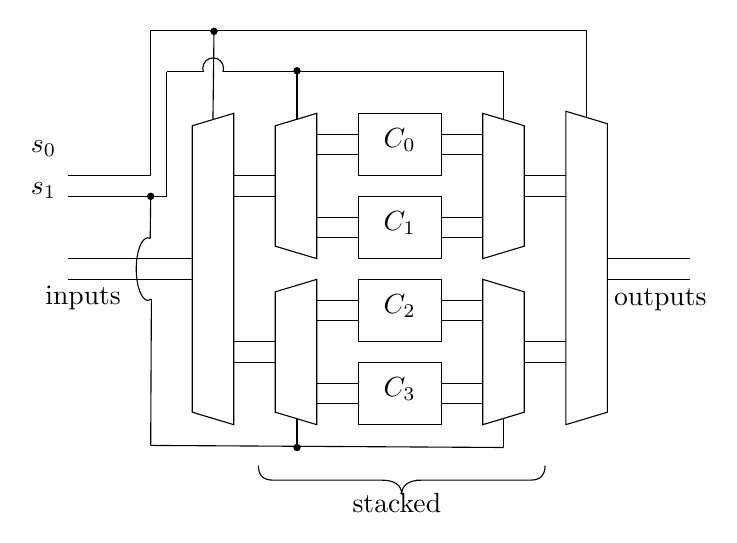
\begin{tikzpicture}[x=0.75pt,y=0.75pt,yscale=-1,xscale=1]
%uncomment if require: \path (0,300); %set diagram left start at 0, and has height of 300

%Shape: Rectangle [id:dp5849077965847459] 
\draw   (330,100) -- (370,100) -- (370,130) -- (330,130) -- cycle ;
%Shape: Rectangle [id:dp07483417235317913] 
\draw   (330,140) -- (370,140) -- (370,170) -- (330,170) -- cycle ;
%Shape: Rectangle [id:dp4166376635287651] 
\draw   (330,180) -- (370,180) -- (370,210) -- (330,210) -- cycle ;
%Shape: Rectangle [id:dp8948354008474025] 
\draw   (330,220) -- (370,220) -- (370,250) -- (330,250) -- cycle ;
%Shape: Trapezoid [id:dp4540566847726426] 
\draw   (310,170) -- (290,164) -- (290,106) -- (310,100) -- cycle ;
%Straight Lines [id:da8956407127966497] 
\draw    (310,120) -- (330,120) ;
%Straight Lines [id:da9777100515836975] 
\draw    (310,110) -- (330,110) ;
%Straight Lines [id:da7425735986407294] 
\draw    (310,160) -- (330,160) ;
%Straight Lines [id:da11610382072678038] 
\draw    (310,150) -- (330,150) ;
%Straight Lines [id:da27169680424513776] 
\draw    (310,200) -- (330,200) ;
%Straight Lines [id:da727422130795774] 
\draw    (310,190) -- (330,190) ;
%Straight Lines [id:da209391042823457] 
\draw    (310,240) -- (330,240) ;
%Straight Lines [id:da44658343194865846] 
\draw    (310,230) -- (330,230) ;
%Straight Lines [id:da6142780982072071] 
\draw    (370,120) -- (390,120) ;
%Straight Lines [id:da6226887597311331] 
\draw    (370,110) -- (390,110) ;
%Straight Lines [id:da2664739221488589] 
\draw    (370,160) -- (390,160) ;
%Straight Lines [id:da026874100929834] 
\draw    (370,150) -- (390,150) ;
%Straight Lines [id:da9856263025895075] 
\draw    (370,200) -- (390,200) ;
%Straight Lines [id:da8016895233324299] 
\draw    (370,190) -- (390,190) ;
%Straight Lines [id:da013651076135336226] 
\draw    (370,240) -- (390,240) ;
%Straight Lines [id:da06626402429808187] 
\draw    (370,230) -- (390,230) ;
%Shape: Trapezoid [id:dp4574780651842486] 
\draw   (430,99) -- (450,105) -- (450,244) -- (430,250) -- cycle ;
%Straight Lines [id:da14149950401750877] 
\draw    (190,180) -- (250,180) ;
%Straight Lines [id:da2825534237984859] 
\draw    (190,170) -- (250,170) ;
%Straight Lines [id:da26233199494209225] 
\draw    (450,180) -- (490,180) ;
%Straight Lines [id:da15777944558688706] 
\draw    (450,170) -- (490,170) ;
%Straight Lines [id:da683223825833436] 
\draw    (190,140) -- (237.7,140) ;
%Straight Lines [id:da4217351698536934] 
\draw    (190,130) -- (230,130) ;
%Straight Lines [id:da9042212392696709] 
\draw    (260,103) -- (260.5,60.5) ;
%Shape: Trapezoid [id:dp5029111964216062] 
\draw   (310,250) -- (290,244) -- (290,186) -- (310,180) -- cycle ;
%Shape: Trapezoid [id:dp11848362887830954] 
\draw   (270,250) -- (250,244) -- (250,106) -- (270,100) -- cycle ;
%Shape: Trapezoid [id:dp4334595235977725] 
\draw   (390,100) -- (410,106) -- (410,164) -- (390,170) -- cycle ;
%Shape: Trapezoid [id:dp47262860257177874] 
\draw   (390,180) -- (410,186) -- (410,244) -- (390,250) -- cycle ;
%Straight Lines [id:da06426061609854339] 
\draw    (270,140) -- (290,140) ;
%Straight Lines [id:da21518984477524328] 
\draw    (270,130) -- (290,130) ;
%Straight Lines [id:da2852878452340667] 
\draw    (270,220) -- (290,220) ;
%Straight Lines [id:da83134608540614] 
\draw    (270,210) -- (290,210) ;
%Straight Lines [id:da4494574594480205] 
\draw    (410,220) -- (430,220) ;
%Straight Lines [id:da1998395845247215] 
\draw    (410,210) -- (430,210) ;
%Straight Lines [id:da8502911411231295] 
\draw    (410,140) -- (430,140) ;
%Straight Lines [id:da7117267186463382] 
\draw    (410,130) -- (430,130) ;
%Straight Lines [id:da17708779177622558] 
\draw    (230,60) -- (230,130) ;
%Straight Lines [id:da9403642725033405] 
\draw    (440,60) -- (413.64,60) -- (230,60) ;
%Straight Lines [id:da7042497085459944] 
\draw    (440,102) -- (440,60) ;
%Straight Lines [id:da02805679708561859] 
\draw    (237.7,80) -- (237.7,140) ;
%Straight Lines [id:da07817997121553377] 
\draw    (255.4,80) -- (237.7,80) ;
%Shape: Arc [id:dp44239178337134166] 
\draw  [draw opacity=0] (255.4,80) .. controls (255.21,79.47) and (255.1,78.89) .. (255.1,78.29) .. controls (255.1,75.53) and (257.34,73.29) .. (260.1,73.29) .. controls (262.86,73.29) and (265.1,75.53) .. (265.1,78.29) .. controls (265.1,78.89) and (264.99,79.47) .. (264.8,80) -- (260.1,78.29) -- cycle ; \draw   (255.4,80) .. controls (255.21,79.47) and (255.1,78.89) .. (255.1,78.29) .. controls (255.1,75.53) and (257.34,73.29) .. (260.1,73.29) .. controls (262.86,73.29) and (265.1,75.53) .. (265.1,78.29) .. controls (265.1,78.89) and (264.99,79.47) .. (264.8,80) ;
%Straight Lines [id:da536984199276638] 
\draw    (400,80) -- (264.8,80) ;
%Straight Lines [id:da9432174552358485] 
\draw    (400,103) -- (400,80) ;
%Straight Lines [id:da35579058464398416] 
\draw    (300.5,261) -- (300.5,247) ;
%Straight Lines [id:da2050986286068066] 
\draw    (400,261) -- (400,247) ;
%Straight Lines [id:da19791404796609613] 
\draw    (400,261) -- (230,260) ;
%Straight Lines [id:da09964823261578626] 
\draw    (230,140) -- (229.77,160.29) ;
%Shape: Arc [id:dp5324078769456657] 
\draw  [draw opacity=0] (230.34,189.49) .. controls (229.83,189.91) and (229.28,190.13) .. (228.72,190.13) .. controls (225.61,190.14) and (223.07,183.4) .. (223.04,175.07) .. controls (223.02,166.75) and (225.52,159.99) .. (228.64,159.98) .. controls (229.03,159.98) and (229.41,160.09) .. (229.77,160.29) -- (228.68,175.06) -- cycle ; \draw   (230.34,189.49) .. controls (229.83,189.91) and (229.28,190.13) .. (228.72,190.13) .. controls (225.61,190.14) and (223.07,183.4) .. (223.04,175.07) .. controls (223.02,166.75) and (225.52,159.99) .. (228.64,159.98) .. controls (229.03,159.98) and (229.41,160.09) .. (229.77,160.29) ;
%Straight Lines [id:da5048114542451922] 
\draw    (230.34,189.49) -- (230,260) ;
%Shape: Circle [id:dp9836025716711807] 
\draw  [fill={rgb, 255:red, 0; green, 0; blue, 0 }  ,fill opacity=1 ] (228.5,140) .. controls (228.5,139.17) and (229.17,138.5) .. (230,138.5) .. controls (230.83,138.5) and (231.5,139.17) .. (231.5,140) .. controls (231.5,140.83) and (230.83,141.5) .. (230,141.5) .. controls (229.17,141.5) and (228.5,140.83) .. (228.5,140) -- cycle ;
%Shape: Circle [id:dp135415838144737] 
\draw  [fill={rgb, 255:red, 0; green, 0; blue, 0 }  ,fill opacity=1 ] (299,261) .. controls (299,260.17) and (299.67,259.5) .. (300.5,259.5) .. controls (301.33,259.5) and (302,260.17) .. (302,261) .. controls (302,261.83) and (301.33,262.5) .. (300.5,262.5) .. controls (299.67,262.5) and (299,261.83) .. (299,261) -- cycle ;
%Shape: Circle [id:dp8636057586751603] 
\draw  [fill={rgb, 255:red, 0; green, 0; blue, 0 }  ,fill opacity=1 ] (299,79.5) .. controls (299,78.67) and (299.67,78) .. (300.5,78) .. controls (301.33,78) and (302,78.67) .. (302,79.5) .. controls (302,80.33) and (301.33,81) .. (300.5,81) .. controls (299.67,81) and (299,80.33) .. (299,79.5) -- cycle ;
%Straight Lines [id:da041429861674520674] 
\draw    (300.5,103) -- (300.5,81) ;
%Shape: Circle [id:dp005195803815501665] 
\draw  [fill={rgb, 255:red, 0; green, 0; blue, 0 }  ,fill opacity=1 ] (259,60.5) .. controls (259,59.67) and (259.67,59) .. (260.5,59) .. controls (261.33,59) and (262,59.67) .. (262,60.5) .. controls (262,61.33) and (261.33,62) .. (260.5,62) .. controls (259.67,62) and (259,61.33) .. (259,60.5) -- cycle ;
%Shape: Brace [id:dp3838971664751233] 
\draw   (281.88,269.72) .. controls (281.88,274.39) and (284.21,276.72) .. (288.88,276.72) -- (340.94,276.72) .. controls (347.61,276.72) and (350.94,279.05) .. (350.94,283.72) .. controls (350.94,279.05) and (354.27,276.72) .. (360.94,276.72)(357.94,276.72) -- (413,276.72) .. controls (417.67,276.72) and (420,274.39) .. (420,269.72) ;

% Text Node
\draw (341,105.93) node [anchor=north west][inner sep=0.75pt]   [align=left] {$\displaystyle C_{0}$};
% Text Node
\draw (341,145.93) node [anchor=north west][inner sep=0.75pt]   [align=left] {$\displaystyle C_{1}$};
% Text Node
\draw (341,185.93) node [anchor=north west][inner sep=0.75pt]   [align=left] {$\displaystyle C_{2}$};
% Text Node
\draw (341,225.93) node [anchor=north west][inner sep=0.75pt]   [align=left] {$\displaystyle C_{3}$};
% Text Node
\draw (178,181.93) node [anchor=north west][inner sep=0.75pt]   [align=left] {inputs};
% Text Node
\draw (452,182.93) node [anchor=north west][inner sep=0.75pt]   [align=left] {outputs};
% Text Node
\draw (171,111.93) node [anchor=north west][inner sep=0.75pt]   [align=left] {$\displaystyle s_{0}$};
% Text Node
\draw (171,131.93) node [anchor=north west][inner sep=0.75pt]   [align=left] {$\displaystyle s_{1}$};
% Text Node
\draw (326,281.93) node [anchor=north west][inner sep=0.75pt]   [align=left] {stacked};


\end{tikzpicture}


  \caption{%
    The na\"ive stacking of four circuits.
    Conditionals are nested two levels deep; per the \stack algorithm,
    this forces the players to recursively emulate themselves which
    leads to quadratic cost in the number of branches for both players.
  }\label{fig:nested}
\end{figure*}


\begin{figure*}[t]
  \centering
  

\tikzset{every picture/.style={line width=0.75pt}} %set default line width to 0.75pt        

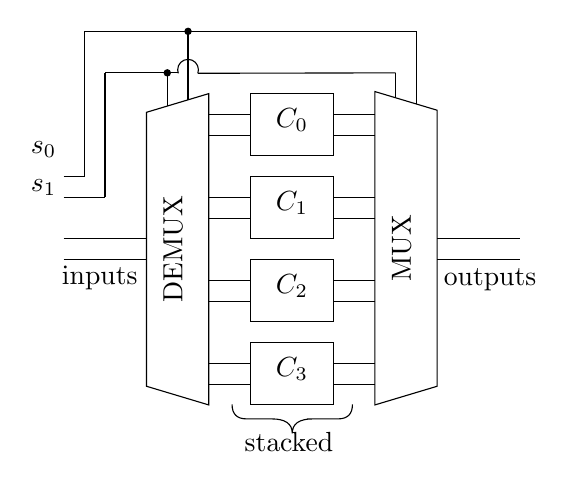
\begin{tikzpicture}[x=0.75pt,y=0.75pt,yscale=-1,xscale=1]
%uncomment if require: \path (0,300); %set diagram left start at 0, and has height of 300

%Shape: Rectangle [id:dp048587029840014395] 
\draw   (120,40) -- (160,40) -- (160,70) -- (120,70) -- cycle ;
%Shape: Rectangle [id:dp5776713339273196] 
\draw   (120,80) -- (160,80) -- (160,110) -- (120,110) -- cycle ;
%Shape: Rectangle [id:dp6797954191886235] 
\draw   (120,120) -- (160,120) -- (160,150) -- (120,150) -- cycle ;
%Shape: Rectangle [id:dp13612273639531247] 
\draw   (120,160) -- (160,160) -- (160,190) -- (120,190) -- cycle ;
%Shape: Trapezoid [id:dp8246309150363402] 
\draw   (100,190) -- (70,181) -- (70,49) -- (100,40) -- cycle ;
%Straight Lines [id:da7525185807979242] 
\draw    (100,60) -- (120,60) ;
%Straight Lines [id:da31461604940557963] 
\draw    (100,50) -- (120,50) ;
%Straight Lines [id:da25486541008995456] 
\draw    (100,100) -- (120,100) ;
%Straight Lines [id:da0077951778335063615] 
\draw    (100,90) -- (120,90) ;
%Straight Lines [id:da2905976026522047] 
\draw    (100,140) -- (120,140) ;
%Straight Lines [id:da7452387399270697] 
\draw    (100,130) -- (120,130) ;
%Straight Lines [id:da0007664179468291898] 
\draw    (100,180) -- (120,180) ;
%Straight Lines [id:da10206153239828308] 
\draw    (100,170) -- (120,170) ;
%Straight Lines [id:da762851249257401] 
\draw    (160,60) -- (180,60) ;
%Straight Lines [id:da7906149158989283] 
\draw    (160,50) -- (180,50) ;
%Straight Lines [id:da7502678160942512] 
\draw    (160,100) -- (180,100) ;
%Straight Lines [id:da9029629905302936] 
\draw    (160,90) -- (180,90) ;
%Straight Lines [id:da3474710624597941] 
\draw    (160,140) -- (180,140) ;
%Straight Lines [id:da15085166543146156] 
\draw    (160,130) -- (180,130) ;
%Straight Lines [id:da33183615362638585] 
\draw    (160,180) -- (180,180) ;
%Straight Lines [id:da3689964414613789] 
\draw    (160,170) -- (180,170) ;
%Shape: Trapezoid [id:dp3485611043917566] 
\draw   (180,39) -- (210,48) -- (210,181) -- (180,190) -- cycle ;
%Straight Lines [id:da03742821351482728] 
\draw    (30,120) -- (70,120) ;
%Straight Lines [id:da7640218221254925] 
\draw    (30,110) -- (70,110) ;
%Straight Lines [id:da956984886166125] 
\draw    (210,120) -- (250,120) ;
%Straight Lines [id:da3748285907762332] 
\draw    (210,110) -- (250,110) ;
%Straight Lines [id:da9714588986108855] 
\draw    (30,90) -- (50,90) ;
%Straight Lines [id:da8529976703877445] 
\draw    (30,80) -- (40,80) ;
%Straight Lines [id:da30690121561733863] 
\draw    (50,30) -- (50,90) ;
%Straight Lines [id:da15914818103441886] 
\draw    (85,30) -- (50,30) ;
%Straight Lines [id:da11238885987153702] 
\draw    (80,30) -- (80,46) ;
%Straight Lines [id:da3144505075089207] 
\draw    (40,10) -- (40,80) ;
%Straight Lines [id:da8817997683520893] 
\draw    (200,10) -- (40,10) ;
%Straight Lines [id:da4268960799866157] 
\draw    (90,43) -- (90,10) ;
%Shape: Arc [id:dp9375967782263986] 
\draw  [draw opacity=0] (85.3,30.21) .. controls (85.11,29.68) and (85,29.1) .. (85,28.5) .. controls (85,25.74) and (87.24,23.5) .. (90,23.5) .. controls (92.76,23.5) and (95,25.74) .. (95,28.5) .. controls (95,29.1) and (94.89,29.68) .. (94.7,30.21) -- (90,28.5) -- cycle ; \draw   (85.3,30.21) .. controls (85.11,29.68) and (85,29.1) .. (85,28.5) .. controls (85,25.74) and (87.24,23.5) .. (90,23.5) .. controls (92.76,23.5) and (95,25.74) .. (95,28.5) .. controls (95,29.1) and (94.89,29.68) .. (94.7,30.21) ;
%Straight Lines [id:da20395268049972604] 
\draw    (190,30) -- (94.7,30.21) ;
%Straight Lines [id:da9984121684679509] 
\draw    (190,42) -- (190,30) ;
%Straight Lines [id:da8655654304921162] 
\draw    (200,45) -- (200,10) ;
%Shape: Circle [id:dp15675574970767925] 
\draw  [fill={rgb, 255:red, 0; green, 0; blue, 0 }  ,fill opacity=1 ] (78.5,30) .. controls (78.5,29.17) and (79.17,28.5) .. (80,28.5) .. controls (80.83,28.5) and (81.5,29.17) .. (81.5,30) .. controls (81.5,30.83) and (80.83,31.5) .. (80,31.5) .. controls (79.17,31.5) and (78.5,30.83) .. (78.5,30) -- cycle ;
%Shape: Circle [id:dp007756137419556719] 
\draw  [fill={rgb, 255:red, 0; green, 0; blue, 0 }  ,fill opacity=1 ] (88.5,10) .. controls (88.5,9.17) and (89.17,8.5) .. (90,8.5) .. controls (90.83,8.5) and (91.5,9.17) .. (91.5,10) .. controls (91.5,10.83) and (90.83,11.5) .. (90,11.5) .. controls (89.17,11.5) and (88.5,10.83) .. (88.5,10) -- cycle ;
%Shape: Brace [id:dp3366641720684751] 
\draw   (111.21,189.72) .. controls (111.21,194.39) and (113.54,196.72) .. (118.21,196.72) -- (130.21,196.72) .. controls (136.88,196.72) and (140.21,199.05) .. (140.21,203.72) .. controls (140.21,199.05) and (143.54,196.72) .. (150.21,196.72)(147.21,196.72) -- (162.21,196.72) .. controls (166.88,196.72) and (169.21,194.39) .. (169.21,189.72) ;

% Text Node
\draw (131,45.93) node [anchor=north west][inner sep=0.75pt]   [align=left] {$\displaystyle C_{0}$};
% Text Node
\draw (131,85.93) node [anchor=north west][inner sep=0.75pt]   [align=left] {$\displaystyle C_{1}$};
% Text Node
\draw (131,125.93) node [anchor=north west][inner sep=0.75pt]   [align=left] {$\displaystyle C_{2}$};
% Text Node
\draw (131,165.93) node [anchor=north west][inner sep=0.75pt]   [align=left] {$\displaystyle C_{3}$};
% Text Node
\draw (13,61.93) node [anchor=north west][inner sep=0.75pt]   [align=left] {$\displaystyle s_{0}$};
% Text Node
\draw (13,79.93) node [anchor=north west][inner sep=0.75pt]   [align=left] {$\displaystyle s_{1}$};
% Text Node
\draw (76.93,142) node [anchor=north west][inner sep=0.75pt]  [rotate=-270] [align=left] {DEMUX};
% Text Node
\draw (186.93,132) node [anchor=north west][inner sep=0.75pt]  [rotate=-270] [align=left] {MUX};
% Text Node
\draw (28,121.93) node [anchor=north west][inner sep=0.75pt]   [align=left] {inputs};
% Text Node
\draw (212,122.93) node [anchor=north west][inner sep=0.75pt]   [align=left] {outputs};
% Text Node
\draw (116,201.93) node [anchor=north west][inner sep=0.75pt]   [align=left] {stacked};


\end{tikzpicture}


  \caption{%
    The vectorized stacking of four circuits.
    The evaluator pays only linear cost to evaluate all four branches,
    but the generator pays quadratic cost in the number of branches.
  }\label{fig:vector}
\end{figure*}

\begin{figure*}[t]
  \centering
  

\tikzset{every picture/.style={line width=0.75pt}} %set default line width to 0.75pt        

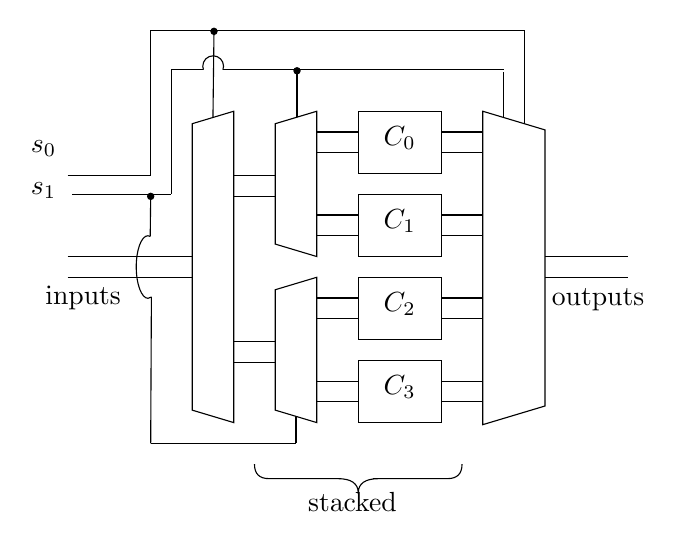
\begin{tikzpicture}[x=0.75pt,y=0.75pt,yscale=-1,xscale=1]
%uncomment if require: \path (0,300); %set diagram left start at 0, and has height of 300

%Shape: Rectangle [id:dp7502614750914376] 
\draw   (330,70) -- (370,70) -- (370,100) -- (330,100) -- cycle ;
%Shape: Rectangle [id:dp7892095271383508] 
\draw   (330,110) -- (370,110) -- (370,140) -- (330,140) -- cycle ;
%Shape: Rectangle [id:dp37989812087032515] 
\draw   (330,150) -- (370,150) -- (370,180) -- (330,180) -- cycle ;
%Shape: Rectangle [id:dp8447591317033223] 
\draw   (330,190) -- (370,190) -- (370,220) -- (330,220) -- cycle ;
%Shape: Trapezoid [id:dp7771424519284856] 
\draw   (310,140) -- (290,134) -- (290,76) -- (310,70) -- cycle ;
%Straight Lines [id:da40802590861909493] 
\draw    (310,90) -- (330,90) ;
%Straight Lines [id:da0031513249223092954] 
\draw    (310,80) -- (330,80) ;
%Straight Lines [id:da1966346673154652] 
\draw    (310,130) -- (330,130) ;
%Straight Lines [id:da6775587210008136] 
\draw    (310,120) -- (330,120) ;
%Straight Lines [id:da12476780588871761] 
\draw    (310,170) -- (330,170) ;
%Straight Lines [id:da9491489855937013] 
\draw    (310,160) -- (330,160) ;
%Straight Lines [id:da6623212585189078] 
\draw    (310,210) -- (330,210) ;
%Straight Lines [id:da6648228335361426] 
\draw    (310,200) -- (330,200) ;
%Straight Lines [id:da31517601583694976] 
\draw    (370,90) -- (390,90) ;
%Straight Lines [id:da6109875647488371] 
\draw    (370,80) -- (390,80) ;
%Straight Lines [id:da2903769623535476] 
\draw    (370,130) -- (390,130) ;
%Straight Lines [id:da8132090709679021] 
\draw    (370,120) -- (390,120) ;
%Straight Lines [id:da013751964941568051] 
\draw    (370,170) -- (390,170) ;
%Straight Lines [id:da6136724266425235] 
\draw    (370,160) -- (390,160) ;
%Straight Lines [id:da7543906971257488] 
\draw    (370,210) -- (390,210) ;
%Straight Lines [id:da5716941479183147] 
\draw    (370,200) -- (390,200) ;
%Shape: Trapezoid [id:dp7120836027835779] 
\draw   (390,70) -- (420,79) -- (420,212) -- (390,221) -- cycle ;
%Straight Lines [id:da01879494240947388] 
\draw    (190,150) -- (250,150) ;
%Straight Lines [id:da3304230275195208] 
\draw    (190,140) -- (250,140) ;
%Straight Lines [id:da1589324558664057] 
\draw    (420,150) -- (460,150) ;
%Straight Lines [id:da07702618181652965] 
\draw    (420,140) -- (460,140) ;
%Straight Lines [id:da6019545366973683] 
\draw    (192.3,110) -- (240,110) ;
%Straight Lines [id:da052523258101502934] 
\draw    (190,101) -- (230,101) ;
%Straight Lines [id:da10206301164150533] 
\draw    (260,73) -- (260.5,31.5) ;
%Shape: Trapezoid [id:dp5014208697738474] 
\draw   (310,220) -- (290,214) -- (290,156) -- (310,150) -- cycle ;
%Shape: Trapezoid [id:dp0033451661221245432] 
\draw   (270,220) -- (250,214) -- (250,76) -- (270,70) -- cycle ;
%Straight Lines [id:da6917927216058005] 
\draw    (270,111) -- (290,111) ;
%Straight Lines [id:da44243639909608434] 
\draw    (270,101) -- (290,101) ;
%Straight Lines [id:da48193219658000075] 
\draw    (270,191) -- (290,191) ;
%Straight Lines [id:da17896325371154065] 
\draw    (270,181) -- (290,181) ;
%Straight Lines [id:da693911481564593] 
\draw    (230,31) -- (230,101) ;
%Straight Lines [id:da6506643552967423] 
\draw    (410,31) -- (230,31) ;
%Straight Lines [id:da8713257514230749] 
\draw    (410,76) -- (410,31) ;
%Straight Lines [id:da3595596964731239] 
\draw    (240,50) -- (240,110) ;
%Straight Lines [id:da23325573067210137] 
\draw    (255,50) -- (240,50) ;
%Shape: Arc [id:dp43363746138961945] 
\draw  [draw opacity=0] (255.4,50) .. controls (255.21,49.47) and (255.1,48.89) .. (255.1,48.29) .. controls (255.1,45.53) and (257.34,43.29) .. (260.1,43.29) .. controls (262.86,43.29) and (265.1,45.53) .. (265.1,48.29) .. controls (265.1,48.89) and (264.99,49.47) .. (264.8,50) -- (260.1,48.29) -- cycle ; \draw   (255.4,50) .. controls (255.21,49.47) and (255.1,48.89) .. (255.1,48.29) .. controls (255.1,45.53) and (257.34,43.29) .. (260.1,43.29) .. controls (262.86,43.29) and (265.1,45.53) .. (265.1,48.29) .. controls (265.1,48.89) and (264.99,49.47) .. (264.8,50) ;
%Straight Lines [id:da664339624976211] 
\draw    (400,50) -- (264.8,50) ;
%Straight Lines [id:da8087120147451838] 
\draw    (400,73) -- (400,51) ;
%Straight Lines [id:da400002248946426] 
\draw    (300,230) -- (300,217) ;
%Straight Lines [id:da5824042733318846] 
\draw    (300,230) -- (230,230) ;
%Straight Lines [id:da44616987205982805] 
\draw    (230,111) -- (229.77,130.29) ;
%Shape: Arc [id:dp23272127004968368] 
\draw  [draw opacity=0] (230.34,159.49) .. controls (229.83,159.91) and (229.28,160.13) .. (228.72,160.13) .. controls (225.61,160.14) and (223.07,153.4) .. (223.04,145.07) .. controls (223.02,136.75) and (225.52,129.99) .. (228.64,129.98) .. controls (229.03,129.98) and (229.41,130.09) .. (229.77,130.29) -- (228.68,145.06) -- cycle ; \draw   (230.34,159.49) .. controls (229.83,159.91) and (229.28,160.13) .. (228.72,160.13) .. controls (225.61,160.14) and (223.07,153.4) .. (223.04,145.07) .. controls (223.02,136.75) and (225.52,129.99) .. (228.64,129.98) .. controls (229.03,129.98) and (229.41,130.09) .. (229.77,130.29) ;
%Straight Lines [id:da9791876678321777] 
\draw    (230.34,159.49) -- (230,230) ;
%Shape: Circle [id:dp034644651933813386] 
\draw  [fill={rgb, 255:red, 0; green, 0; blue, 0 }  ,fill opacity=1 ] (228.5,111) .. controls (228.5,110.17) and (229.17,109.5) .. (230,109.5) .. controls (230.83,109.5) and (231.5,110.17) .. (231.5,111) .. controls (231.5,111.83) and (230.83,112.5) .. (230,112.5) .. controls (229.17,112.5) and (228.5,111.83) .. (228.5,111) -- cycle ;
%Shape: Circle [id:dp9201679931345544] 
\draw  [fill={rgb, 255:red, 0; green, 0; blue, 0 }  ,fill opacity=1 ] (299,50.5) .. controls (299,49.67) and (299.67,49) .. (300.5,49) .. controls (301.33,49) and (302,49.67) .. (302,50.5) .. controls (302,51.33) and (301.33,52) .. (300.5,52) .. controls (299.67,52) and (299,51.33) .. (299,50.5) -- cycle ;
%Straight Lines [id:da30693031106532875] 
\draw    (300.5,73) -- (300.5,52) ;
%Shape: Circle [id:dp5158540745153025] 
\draw  [fill={rgb, 255:red, 0; green, 0; blue, 0 }  ,fill opacity=1 ] (259,31.5) .. controls (259,30.67) and (259.67,30) .. (260.5,30) .. controls (261.33,30) and (262,30.67) .. (262,31.5) .. controls (262,32.33) and (261.33,33) .. (260.5,33) .. controls (259.67,33) and (259,32.33) .. (259,31.5) -- cycle ;
%Shape: Brace [id:dp7057588613218542] 
\draw   (280,240) .. controls (280,244.67) and (282.33,247) .. (287,247) -- (320,247) .. controls (326.67,247) and (330,249.33) .. (330,254) .. controls (330,249.33) and (333.33,247) .. (340,247)(337,247) -- (373,247) .. controls (377.67,247) and (380,244.67) .. (380,240) ;

% Text Node
\draw (341,75.93) node [anchor=north west][inner sep=0.75pt]   [align=left] {$\displaystyle C_{0}$};
% Text Node
\draw (341,115.93) node [anchor=north west][inner sep=0.75pt]   [align=left] {$\displaystyle C_{1}$};
% Text Node
\draw (341,155.93) node [anchor=north west][inner sep=0.75pt]   [align=left] {$\displaystyle C_{2}$};
% Text Node
\draw (341,195.93) node [anchor=north west][inner sep=0.75pt]   [align=left] {$\displaystyle C_{3}$};
% Text Node
\draw (178,152.93) node [anchor=north west][inner sep=0.75pt]   [align=left] {inputs};
% Text Node
\draw (422,153.93) node [anchor=north west][inner sep=0.75pt]   [align=left] {outputs};
% Text Node
\draw (171,82.93) node [anchor=north west][inner sep=0.75pt]   [align=left] {$\displaystyle s_{0}$};
% Text Node
\draw (171,102.93) node [anchor=north west][inner sep=0.75pt]   [align=left] {$\displaystyle s_{1}$};
% Text Node
\draw (304.63,252.21) node [anchor=north west][inner sep=0.75pt]   [align=left] {stacked};


\end{tikzpicture}


  \caption{%
    Our stacking optimization.
    The four conditional branches are stacked by nesting, but the
    multiplexer is not stacked.
    By leaving the multiplexer unstacked, we prevent the players from
    recursively emulating themselves at quadratic cost.
  }\label{fig:optimized}
\end{figure*}


\begin{figure*}[t]
  \centering
  

\tikzset{every picture/.style={line width=0.75pt}} %set default line width to 0.75pt        

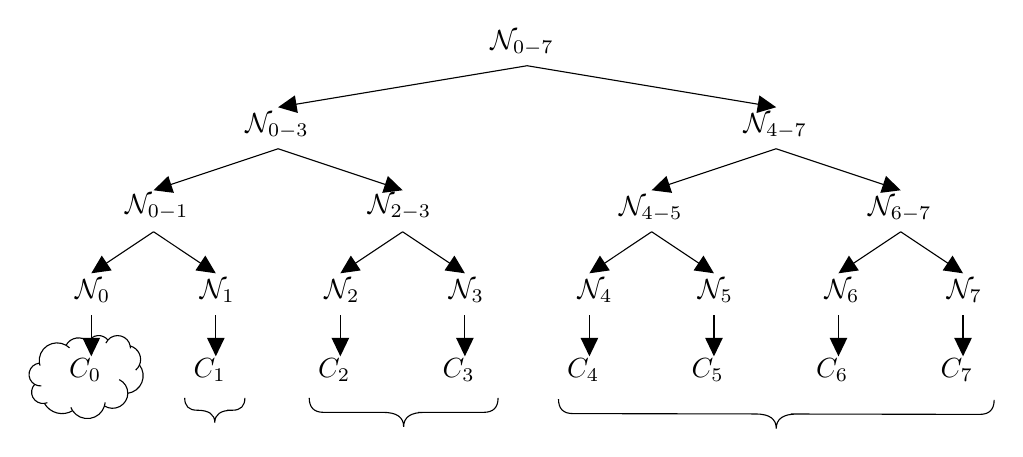
\begin{tikzpicture}[x=0.75pt,y=0.75pt,yscale=-1,xscale=1]
%uncomment if require: \path (0,300); %set diagram left start at 0, and has height of 300

%Straight Lines [id:da6211885505100274] 
\draw    (112.5,168.34) -- (140,150) ;
\draw [shift={(110,170)}, rotate = 326.31] [fill={rgb, 255:red, 0; green, 0; blue, 0 }  ][line width=0.08]  [draw opacity=0] (8.93,-4.29) -- (0,0) -- (8.93,4.29) -- cycle    ;
%Straight Lines [id:da045344571187413196] 
\draw    (140,150) -- (167.5,168.34) ;
\draw [shift={(170,170)}, rotate = 213.69] [fill={rgb, 255:red, 0; green, 0; blue, 0 }  ][line width=0.08]  [draw opacity=0] (8.93,-4.29) -- (0,0) -- (8.93,4.29) -- cycle    ;
%Straight Lines [id:da30999351200098524] 
\draw    (232.5,168.34) -- (260,150) ;
\draw [shift={(230,170)}, rotate = 326.31] [fill={rgb, 255:red, 0; green, 0; blue, 0 }  ][line width=0.08]  [draw opacity=0] (8.93,-4.29) -- (0,0) -- (8.93,4.29) -- cycle    ;
%Straight Lines [id:da0038108532391990524] 
\draw    (260,150) -- (287.5,168.34) ;
\draw [shift={(290,170)}, rotate = 213.69] [fill={rgb, 255:red, 0; green, 0; blue, 0 }  ][line width=0.08]  [draw opacity=0] (8.93,-4.29) -- (0,0) -- (8.93,4.29) -- cycle    ;
%Straight Lines [id:da5202996112606035] 
\draw    (352.5,168.34) -- (380,150) ;
\draw [shift={(350,170)}, rotate = 326.31] [fill={rgb, 255:red, 0; green, 0; blue, 0 }  ][line width=0.08]  [draw opacity=0] (8.93,-4.29) -- (0,0) -- (8.93,4.29) -- cycle    ;
%Straight Lines [id:da44817423034007153] 
\draw    (380,150) -- (407.5,168.34) ;
\draw [shift={(410,170)}, rotate = 213.69] [fill={rgb, 255:red, 0; green, 0; blue, 0 }  ][line width=0.08]  [draw opacity=0] (8.93,-4.29) -- (0,0) -- (8.93,4.29) -- cycle    ;
%Straight Lines [id:da1464427855443573] 
\draw    (472.5,168.34) -- (500,150) ;
\draw [shift={(470,170)}, rotate = 326.31] [fill={rgb, 255:red, 0; green, 0; blue, 0 }  ][line width=0.08]  [draw opacity=0] (8.93,-4.29) -- (0,0) -- (8.93,4.29) -- cycle    ;
%Straight Lines [id:da13582204926626829] 
\draw    (500,150) -- (527.5,168.34) ;
\draw [shift={(530,170)}, rotate = 213.69] [fill={rgb, 255:red, 0; green, 0; blue, 0 }  ][line width=0.08]  [draw opacity=0] (8.93,-4.29) -- (0,0) -- (8.93,4.29) -- cycle    ;
%Straight Lines [id:da30615324718513515] 
\draw    (142.85,129.05) -- (200,110) ;
\draw [shift={(140,130)}, rotate = 341.57] [fill={rgb, 255:red, 0; green, 0; blue, 0 }  ][line width=0.08]  [draw opacity=0] (8.93,-4.29) -- (0,0) -- (8.93,4.29) -- cycle    ;
%Straight Lines [id:da9271896843303857] 
\draw    (200,110) -- (257.15,129.05) ;
\draw [shift={(260,130)}, rotate = 198.43] [fill={rgb, 255:red, 0; green, 0; blue, 0 }  ][line width=0.08]  [draw opacity=0] (8.93,-4.29) -- (0,0) -- (8.93,4.29) -- cycle    ;
%Straight Lines [id:da09808697408042522] 
\draw    (382.85,129.05) -- (440,110) ;
\draw [shift={(380,130)}, rotate = 341.57] [fill={rgb, 255:red, 0; green, 0; blue, 0 }  ][line width=0.08]  [draw opacity=0] (8.93,-4.29) -- (0,0) -- (8.93,4.29) -- cycle    ;
%Straight Lines [id:da8331015133818496] 
\draw    (440,110) -- (497.15,129.05) ;
\draw [shift={(500,130)}, rotate = 198.43] [fill={rgb, 255:red, 0; green, 0; blue, 0 }  ][line width=0.08]  [draw opacity=0] (8.93,-4.29) -- (0,0) -- (8.93,4.29) -- cycle    ;
%Straight Lines [id:da898168093393371] 
\draw    (202.96,89.51) -- (320,70) ;
\draw [shift={(200,90)}, rotate = 350.54] [fill={rgb, 255:red, 0; green, 0; blue, 0 }  ][line width=0.08]  [draw opacity=0] (8.93,-4.29) -- (0,0) -- (8.93,4.29) -- cycle    ;
%Straight Lines [id:da13345957320943236] 
\draw    (320,70) -- (437.04,89.51) ;
\draw [shift={(440,90)}, rotate = 189.46] [fill={rgb, 255:red, 0; green, 0; blue, 0 }  ][line width=0.08]  [draw opacity=0] (8.93,-4.29) -- (0,0) -- (8.93,4.29) -- cycle    ;
%Straight Lines [id:da05876416812491858] 
\draw    (110,207) -- (110,190) ;
\draw [shift={(110,210)}, rotate = 270] [fill={rgb, 255:red, 0; green, 0; blue, 0 }  ][line width=0.08]  [draw opacity=0] (8.93,-4.29) -- (0,0) -- (8.93,4.29) -- cycle    ;
%Straight Lines [id:da5654275867640988] 
\draw    (170,207) -- (170,190) ;
\draw [shift={(170,210)}, rotate = 270] [fill={rgb, 255:red, 0; green, 0; blue, 0 }  ][line width=0.08]  [draw opacity=0] (8.93,-4.29) -- (0,0) -- (8.93,4.29) -- cycle    ;
%Straight Lines [id:da31932671168937365] 
\draw    (230,207) -- (230,190) ;
\draw [shift={(230,210)}, rotate = 270] [fill={rgb, 255:red, 0; green, 0; blue, 0 }  ][line width=0.08]  [draw opacity=0] (8.93,-4.29) -- (0,0) -- (8.93,4.29) -- cycle    ;
%Straight Lines [id:da11489740917816627] 
\draw    (290,207) -- (290,190) ;
\draw [shift={(290,210)}, rotate = 270] [fill={rgb, 255:red, 0; green, 0; blue, 0 }  ][line width=0.08]  [draw opacity=0] (8.93,-4.29) -- (0,0) -- (8.93,4.29) -- cycle    ;
%Straight Lines [id:da24817292659767398] 
\draw    (350,207) -- (350,190) ;
\draw [shift={(350,210)}, rotate = 270] [fill={rgb, 255:red, 0; green, 0; blue, 0 }  ][line width=0.08]  [draw opacity=0] (8.93,-4.29) -- (0,0) -- (8.93,4.29) -- cycle    ;
%Straight Lines [id:da5549995270865108] 
\draw    (410,207) -- (410,190) ;
\draw [shift={(410,210)}, rotate = 270] [fill={rgb, 255:red, 0; green, 0; blue, 0 }  ][line width=0.08]  [draw opacity=0] (8.93,-4.29) -- (0,0) -- (8.93,4.29) -- cycle    ;
%Straight Lines [id:da25264418335124195] 
\draw    (470,207) -- (470,190) ;
\draw [shift={(470,210)}, rotate = 270] [fill={rgb, 255:red, 0; green, 0; blue, 0 }  ][line width=0.08]  [draw opacity=0] (8.93,-4.29) -- (0,0) -- (8.93,4.29) -- cycle    ;
%Straight Lines [id:da07214105669651583] 
\draw    (530,207) -- (530,190) ;
\draw [shift={(530,210)}, rotate = 270] [fill={rgb, 255:red, 0; green, 0; blue, 0 }  ][line width=0.08]  [draw opacity=0] (8.93,-4.29) -- (0,0) -- (8.93,4.29) -- cycle    ;
%Shape: Cloud [id:dp5196949234271024] 
\draw   (85.01,213.17) .. controls (84.56,209.94) and (86.02,206.75) .. (88.75,204.95) .. controls (91.48,203.14) and (95.02,203.04) .. (97.85,204.68) .. controls (98.86,202.81) and (100.7,201.51) .. (102.81,201.19) .. controls (104.93,200.87) and (107.07,201.56) .. (108.6,203.05) .. controls (109.45,201.35) and (111.13,200.2) .. (113.04,200.02) .. controls (114.95,199.85) and (116.82,200.66) .. (117.98,202.17) .. controls (119.52,200.36) and (121.98,199.6) .. (124.29,200.22) .. controls (126.6,200.83) and (128.34,202.71) .. (128.77,205.03) .. controls (130.66,205.54) and (132.24,206.84) .. (133.09,208.6) .. controls (133.95,210.35) and (133.99,212.39) .. (133.22,214.18) .. controls (135.08,216.58) and (135.52,219.79) .. (134.36,222.6) .. controls (133.21,225.4) and (130.64,227.39) .. (127.61,227.82) .. controls (127.58,230.46) and (126.12,232.88) .. (123.79,234.15) .. controls (121.46,235.42) and (118.61,235.34) .. (116.35,233.94) .. controls (115.39,237.1) and (112.68,239.42) .. (109.4,239.91) .. controls (106.12,240.39) and (102.85,238.95) .. (101,236.21) .. controls (98.74,237.56) and (96.03,237.95) .. (93.47,237.29) .. controls (90.92,236.63) and (88.74,234.97) .. (87.43,232.7) .. controls (85.12,232.97) and (82.88,231.78) .. (81.83,229.73) .. controls (80.78,227.68) and (81.14,225.19) .. (82.73,223.52) .. controls (80.67,222.31) and (79.62,219.93) .. (80.13,217.6) .. controls (80.63,215.28) and (82.58,213.54) .. (84.96,213.29) ; \draw   (82.73,223.52) .. controls (83.71,224.08) and (84.83,224.34) .. (85.95,224.25)(87.43,232.7) .. controls (87.91,232.64) and (88.38,232.52) .. (88.84,232.35)(101,236.21) .. controls (100.66,235.71) and (100.38,235.16) .. (100.15,234.6)(116.35,233.94) .. controls (116.53,233.37) and (116.64,232.77) .. (116.69,232.17)(127.6,227.82) .. controls (127.63,225.02) and (126.02,222.45) .. (123.47,221.22)(133.22,214.18) .. controls (132.8,215.13) and (132.17,215.98) .. (131.38,216.66)(128.77,205.03) .. controls (128.84,205.42) and (128.87,205.81) .. (128.86,206.2)(117.98,202.17) .. controls (117.59,202.62) and (117.28,203.12) .. (117.04,203.66)(108.6,203.05) .. controls (108.39,203.45) and (108.24,203.89) .. (108.14,204.33)(97.85,204.68) .. controls (98.45,205.03) and (99.01,205.45) .. (99.51,205.93)(85.01,213.17) .. controls (85.07,213.61) and (85.16,214.05) .. (85.29,214.48) ;
%Shape: Brace [id:dp37789584804120313] 
\draw   (335.1,230.59) .. controls (335.09,235.26) and (337.41,237.59) .. (342.08,237.6) -- (430.03,237.77) .. controls (436.7,237.78) and (440.03,240.12) .. (440.02,244.79) .. controls (440.03,240.12) and (443.36,237.8) .. (450.03,237.81)(447.03,237.8) -- (537.99,237.98) .. controls (542.66,237.99) and (544.99,235.66) .. (545,230.99) ;
%Shape: Brace [id:dp3826911569900966] 
\draw   (215,230) .. controls (215,234.67) and (217.33,237) .. (222,237) -- (250.5,237) .. controls (257.17,237) and (260.5,239.33) .. (260.5,244) .. controls (260.5,239.33) and (263.83,237) .. (270.5,237)(267.5,237) -- (299,237) .. controls (303.67,237) and (306,234.67) .. (306,230) ;
%Shape: Brace [id:dp8696613256451281] 
\draw   (155,230) .. controls (155,233.98) and (156.99,235.97) .. (160.97,235.97) -- (160.97,235.97) .. controls (166.66,235.97) and (169.5,237.96) .. (169.5,241.94) .. controls (169.5,237.96) and (172.34,235.97) .. (178.03,235.97)(175.47,235.97) -- (178.03,235.97) .. controls (182.01,235.97) and (184,233.98) .. (184,230) ;

% Text Node
\draw (98,209.93) node [anchor=north west][inner sep=0.75pt]   [align=left] {$\displaystyle C_{0}$};
% Text Node
\draw (218,209.93) node [anchor=north west][inner sep=0.75pt]   [align=left] {$\displaystyle C_{2}$};
% Text Node
\draw (278,209.93) node [anchor=north west][inner sep=0.75pt]   [align=left] {$\displaystyle C_{3}$};
% Text Node
\draw (338,209.93) node [anchor=north west][inner sep=0.75pt]   [align=left] {$\displaystyle C_{4}$};
% Text Node
\draw (398,209.93) node [anchor=north west][inner sep=0.75pt]   [align=left] {$\displaystyle C_{5}$};
% Text Node
\draw (458,209.93) node [anchor=north west][inner sep=0.75pt]   [align=left] {$\displaystyle C_{6}$};
% Text Node
\draw (518,209.93) node [anchor=north west][inner sep=0.75pt]   [align=left] {$\displaystyle C_{7}$};
% Text Node
\draw (101,171.93) node [anchor=north west][inner sep=0.75pt]   [align=left] {$\displaystyle \mathcal{N}_{0}$};
% Text Node
\draw (161,171.93) node [anchor=north west][inner sep=0.75pt]   [align=left] {$\displaystyle \mathcal{N}_{1}$};
% Text Node
\draw (221,171.93) node [anchor=north west][inner sep=0.75pt]   [align=left] {$\displaystyle \mathcal{N}_{2}$};
% Text Node
\draw (281,171.93) node [anchor=north west][inner sep=0.75pt]   [align=left] {$\displaystyle \mathcal{N}_{3}$};
% Text Node
\draw (343,171.93) node [anchor=north west][inner sep=0.75pt]   [align=left] {$\displaystyle \mathcal{N}_{4}$};
% Text Node
\draw (401,171.93) node [anchor=north west][inner sep=0.75pt]   [align=left] {$\displaystyle \mathcal{N}_{5}$};
% Text Node
\draw (462,171.93) node [anchor=north west][inner sep=0.75pt]   [align=left] {$\displaystyle \mathcal{N}_{6}$};
% Text Node
\draw (521,171.93) node [anchor=north west][inner sep=0.75pt]   [align=left] {$\displaystyle \mathcal{N}_{7}$};
% Text Node
\draw (125,130.93) node [anchor=north west][inner sep=0.75pt]   [align=left] {$\displaystyle \mathcal{N}_{0-1}$};
% Text Node
\draw (242,130.93) node [anchor=north west][inner sep=0.75pt]   [align=left] {$\displaystyle \mathcal{N}_{2-3}$};
% Text Node
\draw (363,131.93) node [anchor=north west][inner sep=0.75pt]   [align=left] {$\displaystyle \mathcal{N}_{4-5}$};
% Text Node
\draw (483,131.93) node [anchor=north west][inner sep=0.75pt]   [align=left] {$\displaystyle \mathcal{N}_{6-7}$};
% Text Node
\draw (183,91.93) node [anchor=north west][inner sep=0.75pt]   [align=left] {$\displaystyle \mathcal{N}_{0-3}$};
% Text Node
\draw (423,91.93) node [anchor=north west][inner sep=0.75pt]   [align=left] {$\displaystyle \mathcal{N}_{4-7}$};
% Text Node
\draw (301,51.93) node [anchor=north west][inner sep=0.75pt]   [align=left] {$\displaystyle \mathcal{N}_{0-7}$};
% Text Node
\draw (158,209.93) node [anchor=north west][inner sep=0.75pt]   [align=left] {$\displaystyle C_{1}$};


\end{tikzpicture}


  \caption{%
    Suppose there are $8$ branches $\cir_0$ through $\cir_7$, and
    suppose \E guesses that $\cir_0$ is the taken branch.
    If the taken branch is in the subtree $\cir_4$ through $\cir_7$,
    \E will generate the same garbage material for the entire subtree,
    regardless of which branch is actually taken.
    By extension, $\cir_0$ can only be evaluated against $\log 8 = 3$ garbage
    material strings: one for each sibling subtree (sibling subtrees
    are bracketed).
  }\label{fig:seed-tree}
\end{figure*}


\begin{itemize}
  \item Present in formal detail.
\end{itemize}

\begin{construction}\label{cnstr:ourapproach}
  \ourapproach~is something or other.
  Probably an algorithm(s).
\end{construction}

 \section{The \ourschemelong\ Garbling Scheme}\label{sec:approach}
In this section, we formalize our construction, \ourschemelong.
Throughout this section, consider a conditional circuit with $b$
branches.
For simplicity, we ignore the number input and output wires.

We adopt the above simplification because branching factor is the most interesting
aspect of \ourschemelong. We emphasize that ignoring inputs/outputs
does not hide high costs.
% \ourschemelong scales linearly with the number of gates per branch.
While we scale with the product of the number of inputs and $b$ (and
respectively the product of number of outputs and $b$), the
constants are low.
See \Cref{sec:eval} for evidence of these low constants.
Thus, inputs/outputs are of secondary concern to the circuit size,
which is often far larger than the number of inputs/outputs.

Consider garbled circuits $\gcir_i$ corresponding to each branch
$\cir_i$. Let $\nmat$ be the size of the largest such garbling: $\nmat
= \max_i |\gcir_i|$.
Given branching factor $b$, \ourschemelong\ features:
\begin{itemize}
  \item $O(\nmat)$ communication complexity.
  \item $O(\nmat b \log b)$ time complexity.
  \item $O(\nmat \log b)$ space complexity.
\end{itemize}

In this section, we formalize our algorithms and give proofs of the above
complexities. We postpone proofs of correctness and security to
\Cref{sec:proof}.

\ourschemelong\ is formalized as a \emph{garbling
scheme}~\cite{CCS:BelHoaRog12}.
Garbling schemes abstract the details of GC such that protocols can be written generically.
That is, \ourschemelong is a modular collection of algorithms, not a
protocol.
Our formalization specifically uses the modified garbling scheme
framework of \HK, which separates the \emph{topology} of circuits
(i.e., the concrete circuit description) from circuit material
(i.e., the collections of encryptions needed to securely evaluate the
circuit), an important modification for SGC.

A garbling scheme is a tuple of five algorithms:
\[ (\gev, \gEv, \gGb, \gEn, \gDe) \]
%
\begin{itemize}
  \item \gev\ specifies circuit semantics. For typical approaches that
    consider only low-level gates, \gev\ is often left implicit since its
    implementation is generally understood. We explicate \gev\ to formalize
    conventions of conditional evaluation.
  \item \gEv\ specifies how \E\ securely evaluates the GC.
  \item \gGb\ specifies how \G\ garbles the GC.
  \item \gEn\ and \gDe\ specify the translation of cleartext values
    to/from GC labels. That is, \gEn\ specifies how player
    inputs translate to input labels and \gDe\ specifies how outputs
    labels translate to cleartext outputs.
\end{itemize}
%
Correct garbling schemes ensure that the garbled functions \gGb, \gEn,
\gEv, and \gDe\ achieve the semantics specified by \gev.

Before we present our garbling scheme \ourschemelong, we introduce the
formal syntax of the circuits it manipulates.
Because our focus is conditional branching, we assume
an \emph{underlying garbling scheme} \underscheme.
\underscheme\ is responsible for handling the collections of low level
gates (typically AND and XOR gates) that we refer to as \emph{netlists}.
In our implementation, we instantiate \underscheme\ with the efficient
half-gates scheme of~\cite{EC:ZahRosEva15}.
We do not specify the syntax of netlists, and entirely leave their
handling to \underscheme.
Our circuit syntax is defined inductively:
Let $\cir_0, \cir_1$ be two arbitrary circuits and $\vec \cir$ be a
a vector of arbitrary circuits. The space of
circuits is defined as follows:
\[
  \cir ::= \netlist(\cdot)~|~%
  \conditional(\vec \cir)~|~%
  \sequential(\cir_0, \cir_1)
\]

That is, a circuit is either (1) a netlist, (2) a conditional dispatch
over a vector of circuits (our focus), or (3) a sequence of two
circuits.
Sequences of circuits are necessary to allow arbitrary
control flow.


\begin{figure}
  \begin{adjustwidth}{-0.1\textwidth}{-0.1\textwidth}
  \centering
  \begin{minipage}[t]{0.56\linewidth}
    \begin{align*}
      &\ourscheme.\gev(\cir, \cirinp):\\
      &~~\codecomment{What are the circuit semantics?}\\
      &~~\switch~\cir:\\
      &~~~~\ccase~\netlist(\cdot): \creturn~\underscheme.\gev(\cir, \cirinp)\\
      &~~~~\ccase~\sequential(\cir_0, \cir_1):
      \creturn~\ourscheme.\gev(\cir_1, \ourscheme.\gev(\cir_0,
      \cirinp))\\
      &~~~~\ccase~\conditional(\vec{\cir}):\\
      &~~~~~~\codecomment{split branch index from input}\\
      &~~~~~~\aid\mid\cirinp' \gets \cirinp\\
      &~~~~~~\codecomment{Run the active branch.}\\
      &~~~~~~\creturn~\ourscheme.\gev(\vec{\cir}[\aid], \cirinp')\\
      \\
      &\ourscheme.\gEv(\cir,\mat,\gcirinp):\\
      &~~\codecomment{How does \E evaluate the GC?}\\
      &~~\switch(\cir):\\
      &~~~~\ccase~\netlist(\cdot): \creturn~\underscheme.\gEv(\cir,\mat,\gcirinp)\\
      &~~~~\ccase~\sequential(\cir_0, \cir_1): \\
      &~~~~~~\mat_0\mid\mat_{tr}\mid\mat_1 \gets \mat\\
      &~~~~~~\creturn~\ourscheme.\gEv(\cir_1, \mat_1, \evtranslate(\ourscheme.\gEv(\cir_0, \mat_0, \cirinp), \mat_{tr})\\
      &~~~~\ccase~\conditional(\vec \cir): \creturn~\evcond(\vec \cir,
      \mat, \gcirinp)\\
      \\
      &\ourscheme.\gEn(e,\cirinp):\\
      &~~\codecomment{How do inputs map to labels?}\\
      &~~\codecomment{This works for all projective schemes:}\\
      &~~\gcirinp \gets \emptystring\\
      &~~\cfor~i \in 0..n\minus 1:\\
      &~~~~(X^0, X^1) \gets e[i]\\
      &~~~~\cif~\cirinp[i] = 0:~\{~\gcirinp[i] \gets X^0~\}~\celse:~\{~\gcirinp[i] \gets X^1~\}\\
      &~~\creturn~\gcirinp
    \end{align*}
  \end{minipage}
  %
  \begin{minipage}[t]{0.40\linewidth}
    \begin{align*}
      &\ourscheme.\gGb(1^\kappa, \cir, S)\\
      &~~\codecomment{How does \G garble the GC?}\\
      &~~\codecomment{$S$ is an explicit seed.}\\
      &~~\switch~\cir:\\
      &~~~~\ccase~\netlist(\cdot):\\
      &~~~~~~\creturn~\underscheme.\gGb(1^\kappa,\cir,S)\\
      &~~~~\ccase~\sequential(\cir_0, \cir_1):\\
      &~~~~~~\codecomment{Derive seeds for two circuits.}\\
      &~~~~~~S_0 \gets F_S(0)\\
      &~~~~~~S_1 \gets F_S(1)\\
      &~~~~~~(\mat_0, e_0, d_0) \gets \ourscheme.\gGb(1^\kappa,\cir_0, S_0)\\
      &~~~~~~(\mat_1, e_1, d_1) \gets \ourscheme.\gGb(1^\kappa,\cir_1, S_1)\\
      &~~~~~~\codecomment{Labels out of $\cir_0$ must be \emph{translated}}\\
      &~~~~~~\codecomment{to labels into $\cir_1$.}\\
      &~~~~~~\mat_{tr} \gets \gbtranslate(d_0,e_1)\\
      &~~~~~~\mat \gets \mat_0\mid \mat_{tr}\mid \mat_1\\
      &~~~~~~\creturn~(\mat, e_0, d_1)\\
      &~~~~\ccase~\conditional(\vec \cir): \creturn~\gbcond(\vec \cir, S)\\
      \\
      &\ourscheme.\gDe(d, \gcirout):\\
      &~~\codecomment{How do labels map to outputs?}\\
      &~~\codecomment{This works for all projective schemes:}\\
      &~~\cirout \gets \lambda\\
      &~~\cfor~i \in 0.. m\minus 1:\\
      &~~~~(Y^0, Y^1) \gets d[i]\\
      &~~~~\cif~\gcirout[i] = Y^0:~\cirout[i] \gets 0\\
      &~~~~\celse~\cif~\gcirout[i] = Y^1:~\cirout[i] \gets 1\\
      &~~~~\celse:~\mathtt{ABORT}\\
      &~~\creturn~\cirout
      % &\genprojection(n, S):\\
      % &~~p \gets \lambda\\
      % &~~\cfor~i \in 0..n\minus 1:\\
      % &~~~~X^0 \drawnfrom{S} \{0, 1\}^{\kappa}\\
      % &~~~~X^1 \drawnfrom{S} \{0, 1\}^{\kappa}\\
      % &~~~~c \drawnfrom{S} \{0, 1\}\\
      % &~~~~p \gets p \mid ((X^0\mid c), (X^1\mid \xor{1}{c}))\\
      % &~~\creturn~p
    \end{align*}
  \end{minipage}
  \end{adjustwidth}
  \caption{%
    Our garbling scheme \ourschemelong.
    The included algorithms are typical except for the handling of
    conditionals.
    \gEv\ and \gGb\ delegate the core of our approach the \evcond\ and
    \gbcond\ respectively.
  }\label{fig:scheme}
\end{figure}


With our syntax established, we are ready to present our algorithms.
\begin{construction}[\ourschemelong]\label{ourconstr}
  \ourschemelong\ is the tuple of algorithms:
  \[ (\ourscheme.\gev, \ourscheme.\gEv, \ourscheme.\gGb, \ourscheme.\gEn, \ourscheme.\gDe) \]
  Definitions for each algorithm are listed in \Cref{fig:scheme}.
\end{construction}

\Cref{ourconstr} is proved correct and secure in \Cref{sec:proof}.
Theorems and lemmas in this section imply the following efficiency theorem:
% \begin{theorem}
%   Let $\underscheme$ be a garbling scheme that is
%       \textbf{correct}, \textbf{strongly stackable},
%       \textbf{authentic}, and \textbf{private}.
%   Then \Cref{ourconstr} instantiated with $\underscheme$ is
%       \textbf{correct}, \textbf{strongly stackable},
%       \textbf{authentic}, and \textbf{private}.
% \end{theorem}

\begin{theorem}\label{thm:efficiency}
  Let $\underscheme$ be a garbling scheme satisfying the following
  property:
  \begin{itemize}
    \item Let $\cir$ be an arbitrary netlist and let $s$ be the size of
      material generated by invoking $\underscheme.\gGb$ on $\cir$.
      Let both $\underscheme.\gEv$ and $\underscheme.\gGb$, invoked
      on $\cir$, run in $O(s)$ time and $O(s)$ space.
  \end{itemize}
  Then \Cref{ourconstr} instantiated with $\underscheme$ satisfies the
  following property.
  \begin{itemize}
    \item Let $\vec{\cir}$ be a vector of $b$ arbitrary netlists. Let $\nmat$ be
      the maximum size of the garblings constructed by calling
      $\underscheme.\gGb$ on each of these $b$ netlists.
      Then both $\ourscheme.\gEv$ and $\ourscheme.\gGb$, invoked on
      $\conditional(\vec{\cir})$, run in
      $O(\nmat b \log b)$ time and $O(\nmat \log b$) space.
  \end{itemize}
\end{theorem}

Standard garbling schemes, e.g. the
half-gates scheme~\cite{EC:ZahRosEva15}, achieve the efficiency
required by \Cref{thm:efficiency}, since they simply handle each gate
individually.

We now draw attention to two key details of algorithms in
\Cref{fig:scheme}:
(1) $\ourscheme.\gEv$ delegates to a subprocedure \evcond\ and (2)
$\ourscheme.\gGb$ delegates to a subprocedure \gbcond.
%
All details of conditionals are handled by these two subprocedures.
%
Aside from these delegations, the algorithms in \Cref{fig:scheme} are
relatively unsurprising:
the algorithms closely match \HK's construction and essentially
provide 
%nothing more than 
infrastructure needed to host our contribution.
%
We briefly discuss the most relevant details of these 
%less interesting 
algorithms before returning
to an extended discussion of \evcond\ and \gbcond~(c.f. \Cref{sec:approach-cond}):

\begin{itemize}
  \item \textbf{Projectivity.} \ourschemelong\
    is a \emph{projective garbling scheme}~\cite{CCS:BelHoaRog12}.
    This stronger definition requires that the input \emph{encoding string}
    $e$ and output \emph{decoding string} $d$ have a specific format:
    they must both be a vector of pairs of labels such that the left
    element of each pair is a label encoding logical $0$ and the right
    element of each pair is a label encoding logical $1$.
    Thus, $\ourscheme.\gEn$ and $\ourscheme.\gDe$ are straightforward
    mappings between cleartext values and encoding/decoding strings.
  \item \textbf{Delegation to \underscheme.} Note that
    $\ourscheme.\gev$, $\ourscheme.\gEv$, and $\ourscheme.\gDe$ indeed
    directly delegate to \underscheme\ in the case of a netlist.
  \item \textbf{Sequences and Translation.} In a sequence of two
    circuits, all output wires of the first circuit are passed as the inputs
    to the second. Because these two circuits are garbled starting
    from different seeds, the output labels from $\cir_0$ will not match the required
    input encoding of $\cir_1$.
    %
    We thus implement a \emph{translation} component ($\evtranslate$
    and $\gbtranslate$) that implements via garbled rows
    straightforward translation from one encoding to another.
    \dave{Add note about standard model and PRF to implement
    translation}
\end{itemize}

\subsection{Algorithms for Handling of Conditionals}\label{sec:approach-cond}

With the remaining formalization out of the way, we focus specifically
on conditional branching. Our specific goal is to formalize \evcond\
and \gbcond, the key sub-procedures invoked by $\ourscheme.\gEv$ and
$\ourscheme.\gGb$ respectively.
Note, our presentation is a formalization of the discussion in
\Cref{sec:techOverview}; the following explores the technical aspects
of our construction, but the reader should refer to
\Cref{sec:techOverview} for unifying high level intuition.

\subsubsection{Demultiplexer and Multiplexer.}

Before we discuss handling the body of conditionals, we briefly discuss
entering and leaving a conditional.
%
That is, we describe the \emph{demultiplexer} and \emph{multiplexer}
components.

The demultiplexer component is responsible for (1) forwarding the
conditional inputs to the active branch $\cir_\aid$ and (2) forwarding
garbage inputs to each branch $\cir_{i \neq \aid}$.
Precisely, the demultiplexer computes the following function for
each input $x$ to each branch $\cir_i$:
\begin{align*}
demux(x, i, \aid) =
   \begin{cases}
     x,& \text{if $i = \aid$}\\
     \bot, &\text{otherwise}
   \end{cases}
\end{align*}
where $\bot$ is an arbitrary constant value.
In the GC, the label corresponding to $\bot$ is independent yet
indistinguishable from the corresponding $0$ and $1$ labels (for
security, it is crucial that this value is independent).
The demultiplexer is easily implemented by garbled rows.
The number of required rows is proportional to the number of branches
and the number of branch inputs.
%
\evcond\ and \gbcond\ make use of \evdem\ and \gbdem, procedures which
implement the above function inside GC.
Although we do not, for simplicity, formally describe these, we
emphasize they are the straightforward implementation of garbled rows.

The multiplexer is central to our approach.
It non-interactively eliminates garbage outputs from inactive
branches.
%
Despite its central role, if \G\ knows the garbage
outputs from each branch, the multiplexer's implementation is simple.
%
Specifically, suppose each branch $\cir_i$ has an output $x_i$ that
should propagate if that branch is active.
The multiplexer computes the following function:
\begin{align*}
  mux(x_0, ..., x_{b-1}, \aid) = x_\aid
\end{align*}
Given that (1) each value $x_{i\neq \aid}$ is a fixed constant, at
least with respect to a given \aid, (a
property that we carefully arrange via the demultiplexer) and (2) \G\
knows the value of each of these fixed constants (the central point of
our work), then the above function is easily implemented as a
collection of garbled rows.
The number of required rows is proportional to the number of branches
and the number of conditional outputs.
\evcond\ and \gbcond\ make use of \evmux\ and \gbmux, procedures which
implement the above function inside GC.
Like the demultiplexer, we do not formalize these procedures in
detail, but their implementation is the straightforward handling of
garbled rows.



\subsubsection{Garbling Subtrees.}
\begin{figure}[t!]\centering\framebox{%
\begin{minipage}{0.97\linewidth}
% \begin{figure}[t]
  \begin{align*}
    &\gbtree(\vec{\cir}, i, j, seed):\\
    &~~\cif~i = j:\\
    &~~~~\codecomment{Base case of $1$ branch.}\\
    &~~~~M, e, \cdot \gets \gb(\vec\cir[i], seed)\\
    &~~~~\creturn~M, e\\
    &~~\celse:\\
    &~~~~\codecomment{Expand child seeds using PRF.}\\
    &~~~~seed_L \gets F_{seed}(0)\\
    &~~~~seed_R \gets F_{seed}(1)\\
    &~~~~\codecomment{Recursively garble both child trees and stack
    material.}\\
    &~~~~k \gets \halfway(i, j)\\
    &~~~~M_L, e_L \gets \gbtree(\vec{\cir}, i, k, seed_L)\\
    &~~~~M_R, e_R \gets \gbtree(\vec{\cir}, k + 1, j, seed_R)\\
    &~~~~\creturn~(M_L \oplus M_R, e_L \mid e_R)\\
    \\
    &\halfway(i, j):\\
    &~~\codecomment{Simple helper for splitting range of branches (approximately) in half.}\\
    &~~\creturn~i+\left\lfloor \frac{j-i}{2} \right\rfloor\\
  \end{align*}
\end{minipage}}
  \caption{%
    The helper algorithm \gbtree\ starts from a single seed
    at the root of a subtree $\node_{i,j}$, derives all seeds in the
    subtree, garbles all branches in the subtree, and stacks (using
    XOR) all resultant material. The procedure also returns the input
    encodings for all branches.
  }\label{fig:gbtree}
\end{figure}

Recall, we organize the $b$ branches into a binary branching tree.
% Both \evcond\ and \gbcond\ frequently perform a common task:
% they garble all branches in an entire subtree and stack together all
% material.
For \emph{each} internal node of the tree, both \evcond\ and \gbcond\
perform a common task: they garble all branches in the entire subtree
rooted at that node and stack together all material.
%
We thus start by definining a procedure, \gbtree~(\Cref{fig:gbtree}),
which specifically performs this basic task.

Specifically, \gbtree\ recursively descends through the
subtree starting from its root, uses a PRF to derive child seeds from the parent seed, and at the
leaves garbles the branches.
As the recursion propagates back up the tree, the procedure stacks the
garblings together.
%
The recursion tracks two integers $i$ and
$j$, denoting the range of branches $\cir_i..\cir_j$ that are to
be stacked together.
\evcond\ and \gbcond\ use a similar strategy, and all three algorithms
maintain an invariant that $i,j$ refers to a valid node $\node_{i,j}$ in the binary
branching tree over the $b$ branches (c.f. \Cref{fig:gbtree} for an
example).
%
Note that because \evcond\ and \gbcond\ invoke \gbtree\ at
\emph{every} node, this entails that both procedures garble
each branch $\cir_i$ more than once, but with different seeds.
As discussed in \Cref{sec:techOverview}, this repeated garbling is key
to reducing the total number of possible garbage outputs that \E\
can compute.


Note two performance properties of \gbtree, recalling that we ignore
inputs/outputs and consider branches with maximum
garbling size $\nmat$.
\begin{lemma}\label{lemma:gbtreetime}
  Let $\vec{\cir}$ be a vector of $b$ circuits,
  let $i, j \in \{0, b-1\}$ satisfy $i \leq j$,
  and let $seed \in \{0, 1\}^\kappa$ be an arbitrary string.
  Then $\gbtree(\vec \cir, i, j, seed)$ invokes $\gGb$ $j - i + 1$ times.
\end{lemma}
\begin{proof}
  Immediate. The procedure only invokes $\gGb$ at the base case.
\end{proof}
In other words, the algorithm garbles each branch only once.
Note that while \Cref{lemma:gbtreetime} (and also
\Cref{lemma:gbtreespace}) holds for all $i, j$ we are
only concerned with it holding for $i, j$ that represent valid nodes
in the binary branching tree of circuits.


\begin{lemma}\label{lemma:gbtreespace}
  Let $\vec{\cir}$ be a vector of $b$ circuits,
  let $i, j \in \{0, b-1\}$ satisfy $i \leq j$,
  and let $seed \in \{0, 1\}^\kappa$ be a arbitrary string.
  If $\Gb$ runs in $O(\nmat)$ space,
  then $\gbtree(\vec \cir, i, j, seed)$ runs in $O(\nmat \log (j-i+1))$ space.
\end{lemma}
\begin{proof}
  In the base case, $\gbtree$ invokes $\gb$. By assumption, this runs
  within our space requirement, and generates a garbling of maximum
  size $\nmat$.
  %
  In the general case, $\gbtree$ recursively invokes itself twice.
  After the first call has finished, we must store the
  intermediate result $M_L$.
  %
  Thus, at each recursive call site, we store a string of size
  $O(\nmat)$.
  Because each recursive call divides the range of considered circuits
  in half, the recursive tree has depth $O(\log(j-i+1))$.
  Hence, the total required storage is $O(\nmat \log(j-i+1))$.
\end{proof}

\subsubsection{Evaluating Conditionals.}

\begin{figure}
  \begin{align*}
    &\evcond(\vec{\cir}, \mat, X):\\
    &~~b \gets | \vec{\cir} |\\
    &~~\codecomment{Parse the active branch index from the rest of the
    input.}\\
    &~~\aid \mid X' \gets X\\
    &~~\codecomment{Parse material for gadgets and body of conditional.}\\
    &~~\mat_\gadget \mid \mat_{dem} \mid \mat_{cond} \mid \mat_{mux} \gets \mat\\
    &~~\codecomment{Run $\gadget$ to compute all of \E's seeds.}\\
    &~~\es \gets \gadget.\mathtt{Ev}(\aid, \mat_\gadget)\\
    &~~\codecomment{Run the demultiplexer to compute input for each
    branch $\cir_i$.}\\
    &~~\vec{X}_{cond} \gets \evdem(\aid, X, \mat_{dem})\\
    \\
    &~~\codecomment{We define a recursive subprocedure that evaluates $\cir_i - \cir_j$ using material $\mat$.}\\
    &~~\evcond'(i, j, \mat_{i, j}):\\
    &~~~~\cif~i = j:\\
    &~~~~~~\codecomment{Base case: compute output by evaluating the branch normally.}\\
    &~~~~~~\codecomment{This base case corresponds to $\guess = i$.}\\
    &~~~~~~\codecomment{Accumulate output labels into the vector
    $\gcirout_{cond}$ (for later garbage collection).}\\
    &~~~~~~\gcirout_{cond}[i] \gets \ev(\cir_i, M, \gcirinp_{cond}[i])\\
    &~~~~\celse:\\
    &~~~~~~k \gets \halfway(i, j)\\
    &~~~~~~\codecomment{Garble the right subtree using the available
    seed,}\\
    &~~~~~~\codecomment{unstack, and recursively evaluate the left
    subtree.}\\
    &~~~~~~\mat_{k+1,j}, \cdot \gets \gbtree(\vec{\cir}, k+1, j, \es_{k+1, j})\\
    &~~~~~~\evcond'(i, k, \mat_{i, j} \oplus \mat_{k+1,j})\\
    &~~~~~~\codecomment{Symmetrically evaluate the right subtree.}\\
    &~~~~~~\mat_{i, k}, \cdot \gets \gbtree(\vec{\cir}, i, k, \es_{i,k})\\
    &~~~~~~\evcond'(k+1, j, \mat_{i, j} \oplus \mat_{i, k})\\
    \\
    &~~\codecomment{Start recursive process from the top of the tree.}\\
    &~~\evcond'(0, b-1, M_{cond})\\
    &~~\codecomment{Eliminate garbage and propagate $\vec{Y}_\aid$ via
    the multiplexer.}\\
    &~~\creturn~\evmux(\aid, \vec{Y}_{cond}, M_{mux})
  \end{align*}
  \caption{%
    \E's procedure, \evcond, for evaluating a conditional with $b$ branches.
    \evcond\ evaluates each branch; $b-1$ evaluations
    result in garbage outputs and one (the evaluation of
    $\cir_\aid$) results in valid outputs.
    The multiplexer collects garbage and propagates output from
    $\cir_\aid$.
    \evcond\ involves $b \log b$ calls to \gGb (via \gbtree), and each
    branch evaluation is done with respect to the garbling of that
    branch's sibling subtrees.
  }\label{fig:evcond}
\end{figure}

We now formalize the procedure by which \E\ handles a vector of
conditionals, \evcond~(\Cref{fig:evcond}).
%
\evcond\ primarily delegates to a recursive subprocedure \evcond'.
Other than this delegation, \evcond\ simply invokes $\gadget.\gEv$
to obtain her seeds, invokes \evdem\ to propagate valid inputs to $\cir_\aid$,
and, after evaluating all branches, invokes $\evmux$ to collect
garbage outputs from all $\cir_{i \neq \aid}$.
%
\evcond' is a formalization of the high level procedure described in
\Cref{sec:techOverview}: \E\ recursively descends through the tree,
constructing and unstacking garblings of subtrees in the general case.
%
When she finally reaches the leaf nodes, she simply evaluates.
%
In the base case $i = \aid$, she will have correctly unstacked all
material except $\mat_\aid$ (because she has good seeds for the
sibling roots of \aid), and hence evaluates correctly.
%
All other cases $i \neq \aid$ will lead to garbage outputs that \G\
must compute.

\paragraph{Efficiency:} In terms of time complexity, we start by examining the \emph{concrete}
efficiency on conditionals with $2^k$ branches for some $k$.
%
Of course, the following proof generalizes to a asymptotic efficiency
regardless of the number of branches, but we include the concrete
proof to emphasize the low constants involved.

\begin{lemma}\label{lemma:evcondtime}
  Let $b = 2^k$ for some $k \in \mathbb{N}$.
  Let $\vec{\cir}$ be a vector of $b$ circuits, $\mat$ be a string of
  length $\nmat$, and $\gcirinp$ be a vector of labels of length
  $\inpsize(\conditional(\vec{\cir}))$.
  $\evcond(\vec{\cir}, \mat, \gcirinp)$ calls \gGb\ $b \log b$ times
  and calls \gEv\ $b$ times.
\end{lemma}
\begin{proof}
  First, it is trivial that \gEv\ is called $b$ times: the
  procedure is called only at the base case, which is reached once per
  leaf.

  Second, \gbtree\ is called twice in the general case, each on a
  subtree of half of the current branches.
  %
  For example, at the root \gbtree\ is called on every branch, which, by
  \Cref{lemma:gbtreetime}, implies $b$ calls to \Gb.
  Now consider a binary branching tree whose leaves are the $b$
  branches and whose internal nodes each correspond to
  a recursive invocation of $\evcond'$.
  At every level of the tree, each internal node garbles every
  leaf below it, via \gbtree.
  Hence, every level of the tree entails $b$ calls to \Gb.
  Since the binary branching tree has $\log b$ levels, there are $b
  \log b$ total calls to \Gb.
\end{proof}

By essentially exactly the same argument, one can prove the following
lemma for arbitrary numbers of branches:
\begin{lemma}\label{lemma:evcondtime-general}
  Let $\vec{\cir}$ be a vector of $b$ circuits, $\mat$ be a string of
  length $\nmat$, and $\gcirinp$ be a vector of labels of length
  $\inpsize(\conditional(\vec{\cir}))$.
  $\evcond(\vec{\cir}, \mat, \gcirinp)$ calls \gGb\ $O(b \log b)$ times
  and calls \gEv\ $b$ times.
\end{lemma}

\begin{lemma}\label{lemma:evcondspace}
  Let $\vec{\cir}$ be a vector of $b$ circuits, $\mat$ be a string of
  length $\nmat$, and $\gcirinp$ be a vector of labels of length
  $\inpsize(\conditional(\vec{\cir}))$.
  $\evcond(\vec{\cir}, \mat, \gcirinp)$ runs in $O(\nmat \log b)$ space.
\end{lemma}
\begin{proof}
  Trivial, since no material is stored at recursive call sites.
  Thus the space complexity is inherited from
  \gbtree~(\Cref{lemma:gbtreespace}).
\end{proof}

\subsubsection{Garbling Conditionals.}
\begin{figure}[t!]\centering\framebox{%
\begin{minipage}{0.97\linewidth}
  \begin{align*}
    &\gbcond(\vec{\cir}, S):\\
    &~~b \gets | \vec{\cir} |\\
    &~~\codecomment{Recursively derive all `good' seeds for the entire tree.}\\
    &~~s \gets \mathtt{DeriveSeedTree}(S, b)\\
    &~~\codecomment{Sample an input encoding for the conditional.}\\
    &~~e \gets \genprojection(S, n)\\
    &~~\codecomment{Parse encoding into encoding of $\aid$
    and encoding of rest of input.}\\
    &~~e_\aid\mid e' \gets e\\
    &~~\codecomment{Garble \gadget\ based on the encoding of \aid.}\\
    &~~\codecomment{This outputs material as well as the tree of all
    `bad' seeds $s'$.}\\
    &~~\mat_\gadget, s' \gets \gadget.\mathtt{Gb}(e_\aid, s)\\
    &~~\codecomment{Construct the stacked material and input encodings for each branch.}\\
    &~~M_{cond}, e_{cond} \gets \gbtree(\vec{\cir}, 0, b-1, s_{0, b-1})\\
    &~~\codecomment{The demux conditionally translates the input encoding $e'$}\\ 
    &~~\codecomment{to one of the branch encodings in $e_{cond}$ based on $e_\aid$.}\\
    &~~\mat_{dem}, \Lambda_{in} \gets \gbdem(e_\aid, e', e_{cond})\\
    &~~\codecomment{Compute all possible garbage outputs.}\\
    &~~\Lambda_{out} \gets \computegarbage(\vec{\cir}, M_{cond}, \Lambda_{in}, s, s')\\
    &~~\codecomment{The demultiplexer collects garbage outputs.}\\
    &~~\mat_{mux} \gets \gbmux(e_\aid, d, \vec{d}, \Lambda_{out})\\
    &~~\creturn~(\mat_\gadget \mid \mat_{dem} \mid \mat_{cond} \mid
    \mat_{mux}, e, d)\\
\end{align*}
\end{minipage}}
  \caption{%
    The algorithm for garbling a conditional vector.
    Given $b$ branches, \gbcond\ returns (1) the stacked material, (2)
    the input encoding string, (3) all $b$ output decoding strings,
    and (4) all $b\log b$ possible garbage output label vectors.
  }\label{fig:gbcond}
\end{figure}


\begin{figure}
  \begin{align*}
    &\computegarbage(\vec{\cir}, \mat, \Lambda_{in}, s, s'):\\
    &~~\codecomment{We first define a recursive subprocedure.}\\
    &~~\computegarbage'(i, j, \mat_{i,j}, \vec{\mat}'):\\
    &~~~~\codecomment{Compute all possible garbage outputs from
    branches $\cir_i-\cir_j$.}\\
    &~~~~\codecomment{$\vec{\mat}'$ is a vector of the bad garblings of
      all sibling roots of the current node.}\\
    &~~~~\cif~i = j:\\
    &~~~~~~\codecomment{Base case: loop over all possible garbage material}\\
    &~~~~~~\codecomment{and accumulate garbage outputs into
    $\Lambda_{out}$.}\\
    &~~~~~~acc \gets \mat_{i,i}\\
    &~~~~~~\cfor~k \in 0..|\vec{\mat}'|-1:\\
    &~~~~~~~~\codecomment{Emulate all possible bad evaluations of $\cir_i$.}\\
    &~~~~~~~~acc \gets acc \oplus \vec{\mat}'[k]\\
    &~~~~~~~~\Lambda_{out}[i][k] \gets \gEv(\vec{\cir}[i], acc, \Lambda_{in}[k])\\
    &~~~~\celse:\\
    &~~~~~~k \gets \halfway(i, j)\\
    &~~~~~~\codecomment{Compute the good material for both subtrees.}\\
    &~~~~~~\mat_{i, k}, \cdot \gets \gbtree(\vec{\cir}, i, k, s_{i, k})\\
    &~~~~~~\mat_{k+1, j} \gets \mat_{i, j} \oplus \mat_{i, k}\\
    &~~~~~~\codecomment{Compute the bad material for both subtrees.}\\
    &~~~~~~\mat_{i, k}' \gets \gbtree(\vec{\cir}, i, k, s'_{i, k})\\
    &~~~~~~\mat_{k+1, j}' \gets \gbtree(\vec{\cir}, k+1, j, s'_{k+1, j})\\
    &~~~~~~\codecomment{Recursively compute all garbage outputs.}\\
    &~~~~~~\computegarbage'(i, k, (\mat_{k+1,j} \oplus \mat_{k+1,j}') \mid \vec{\mat}')\\
    &~~~~~~\computegarbage'(k+1, j, (\mat_{i,k} \oplus \mat_{i,k}') \mid \vec{\mat}')\\
    \\
    &~~b \gets |\vec{\cir}|\\
    &~~\codecomment{Start the recursive process using the top level material $\mat$}\\
    &~~\codecomment{and using the empty vector of bad sibling material.}\\
    &~~\computegarbage'(0, b-1, \mat, [~])\\
    &~~\creturn~\Lambda_{out}
  \end{align*}
  \caption{%
    \computegarbage\ allows \G\ to compute the possible garbage output labels
    from evaluation of inactive branches.
    Specifically, the algorithm takes as arguments (1) the vector of
    conditional branches $\vec{\cir}$, (2) the `good' material for the
    conditional $M$, (3) the garbage input labels $\Lambda_{in}$, (4)
    the tree of `good' seeds (i.e. the seeds used by \G\ to generate
    $M$) $s$, and (5) the tree of `bad' seeds $s'$.
    The algorithm outputs $\Lambda_{out}$, the vector (length $b$) of
    vectors (each length $\log b$) of output labels from each
    branch.
  }\label{fig:computegarbage}
\end{figure}

Finally, we formalize \G's procedure for handling vectors of
conditional branches, \gbcond~(\Cref{fig:gbcond}).
%
\begin{enumerate}
  \item \gbcond\ starts by recursively deriving a binary branching tree of
good seeds by calling $\mathtt{DeriveSeedTree}$. This call just uses a PRF
to recursively derive seeds using the standard trick.
%
\item \gbcond\ invokes $\genprojection$ to select a uniform input
encoding $e$: $e$ is the vector of pairs of labels that are
valid input labels for the overall conditional.
%
\item \gbcond\ uses $\gadget.\gGb$ to compute garbled rows for
  $\gadget$ and also to compute all possible `bad' seeds: \G\ needs
  these bad seeds to emulate \E\ when making a bad guess.
%
\item \gbcond\ uses $\gbtree$ to compte the stacked material
$\mat_{cond}$ starting from the root of the seed tree.
$\mat_{cond}$ is the long string that \G\ ultimately sends to \E.
%
\item \gbcond\ calls $\gbdem$ to compute the demultiplexer garbled
  rows.  This call also returns the garbage input labels for each
  branch; essential information that allows \G\ to emulate \E.
\end{enumerate}
With this accomplished, \gbcond's remaining task is to encrypt the
garbage collecting multiplexer.
However, as we have argued throughout this work, it is not clear how
this can be achieved unless \G\ \emph{knows all garbage outputs} that
\E\ might compute.
%
Thus, \gbcond\ first invokes \computegarbage
(\Cref{fig:computegarbage}, a procedure which
emulates all of \E's bad guesses.

\computegarbage\ delegates to the recursive subprocedure
\computegarbage'. This recursive procedure walks down the tree,
maintaining two key variables: (1) $\mat_{i,j}$ holds the correct
material for the current subtree $\node_{i,j}$ and (2) $\vec{\mat}'$
holds a vector of bad materials of the incorrectly garbled sibling
roots of $\node_{i,j}$.
%
In the general case, these variables are simply appropriately updated
via calls to $\gbtree$.
In the base case, the garbage materials for all sibling roots are now
available.
Additionally, all garbage inputs into each branch are available in the
vector $\Lambda_{in}$.
%
Thus, in the base case we can compute all garbage outputs for each
branch by calling \gEv\ on the proper combinations of garbage material
and labels.
%
We store all garbage outputs into the vector $\Lambda_{out}$, which is
returned by the overall procedure, and then ultimately used by
\gbcond\ to call $\gbmux$.

\paragraph{Efficiency:} Like \evcond, we start with a concrete claim
of conditionals branching factors that are powers of two:
\begin{lemma}\label{lemma:gbcondtime}
  Let $b = 2^k$ for $k \in \mathbb{N}$.
  Let $\vec{\cir}$ be a vector of $b$ circuits and $S \in \{0,
  1\}^\kappa$ be a string.
  $\gbcond(\vec{\cir}, S)$ calls \gGb\ $\frac{3}{2}b \log b + b$ times and calls
  $\gEv$ $b\log b$ times.
\end{lemma}
\begin{proof}
  First, we handle the $b$ \gGb\ calls. These $b$ calls arise from the
  top-level call to $\gbtree$ in $\gbcond$.
  The remaining $\frac{3}{2} b \log b$ calls come from
  \computegarbage.
  %
  Our argument is similar to that of \Cref{lemma:evcondtime}:
  at each level of the binary branching tree, $\computegarbage$ calls
  $\gGb$ $\frac{3}{2}b$ times (via each node's three calls to \gbtree\
  on half of the node's ancestors).
  Since there are $\log b$ levels in the tree, $\computegarbage$ calls
  \gGb\ a total of $\frac{3}{2}b \log b$ times.

  All calls to $\gEv$ also arise from $\computegarbage$.
  In particular, $\gEv$ calls occur in the base case (reached once per
  branch).
  Each branch is evaluated $\log b$ times: once per appropriate
  combination of garbage material. Since each leaf has $\log b$
  sibling roots, the vector $\vec{\mat}'$ has $\log b$ members.
  %
  Hence, we invoke $\gEv$ a total of $b \log b$ times.
\end{proof}

By essentially the same argument, the following asymptotic claims holds
for conditionals with arbitrary branching factors:
\begin{lemma}\label{lemma:gbcondtime-general}
  Let $\vec{\cir}$ be a vector of $b$ circuits and $S \in \{0,
  1\}^\kappa$ be a string.
  $\gbcond(\vec{\cir}, S)$ calls \gGb\ $O(b \log b)$ times and calls
  $\gEv$ $O(b\log b)$ times.
\end{lemma}

Finally, \gbcond\ runs in logarithmic space:
\begin{lemma}\label{lemma:gbcondspace}
  Let $\vec{\cir}$ be a vector of $b$ circuits and $S \in \{0, 1\}^\kappa$ be a string.
  If $\gGb$ runs in $O(\nmat)$ space, then
  $\gbcond(\vec{\cir}, S)$ runs in $O(\nmat \log b)$ space.
\end{lemma}
\begin{proof}
  Like $\evcond$, \gbcond\ largely consumes space due to calls to
  $\gbtree$. However, by \Cref{lemma:gbtreespace}, each of these calls
  runs in $O(\nmat \log b)$ space.
  %
  Additionally, \computegarbage\ maintains a vector of material
  $\vec{\mat}'$.
  However, this vector's size is bounded by the depth of the tree: we
  concatenate one material to the vector at each recursive call
  site.
  Hence, $\vec{\mat}'$ holds $O(\log b)$ elements and hence has
  $O(\nmat \log b)$ size.
\end{proof}

\section{Correctness/Security Proofs}\label{sec:proof}

We now prove the relevant properties of \ourschemelong, in particular
showing that it is correct and secure.
We formalize our theorems in the~\cite{CCS:BelHoaRog12} framework,
which requires a candidate garbling scheme to be \textbf{correct},
\textbf{oblivious}, \textbf{private}, and \textbf{authentic}.
This section shows that \ourschemelong\ satisfies these properties.

In addition, \HK\ introduced a new property, \textbf{stackability}, which
formalizes the class of garbling schemes whose garblings can be
securely stacked; hence stackable schemes are candidate underlying
schemes.
%
In this work, we strengthen the definition of stackability.  This
strengthening, which we call \textbf{strong stackability}, allows us to
prove security under standard assumptions (an improvement over \HK,
which required a random oracle assumption).
Strong stackability is strictly stronger than stackability; all
strongly
stackable schemes are stackable,
and all lemmas that hold for stackable schemes hold also for strongly
stackable schemes.
A key application of this second fact is that all stackable schemes
are trivially \textbf{oblivious}, so all strongly stackable schemes are
also oblivious.
We prove security given a strongly stackable scheme.

\HK\ showed that standard garbling schemes are stackable, including
the state-of-the-art half-gates technique~\cite{EC:ZahRosEva15}.
We further argue that such schemes either are strongly stackable without
modification or can be easily adjusted.
Hence, our implementation can assume a RO and use half-gates as its underlying
scheme to achieve high performance.

We also show that \ourschemelong\ is itself strongly stackable, giving
flexibility in usage: while by design \ourschemelong\ handles vectors
of conditional branches, we also support arbitrarily nested
conditional control flow without modifying the source program.
%
We note that this nested usage \emph{does not} give $O(b\log b)$
computation, and so vectorized branches should favored where possible.
% Because \ourschemelong\ is strongly stackable, it is trivially
% \textbf{oblivious}~\HK,
% and so we do not discuss obliviousness further.



\subsection{Correctness}\label{sec:correctness}

\begin{definition}[Correctness]\label{def:correct}
  A garbling scheme is \textbf{correct} if for
  all circuits $\cir$,
  all input strings $\cirinp$ of length $\inpsize(\cir)$,
  and all pseudorandom seeds $S$:
  \[
    \gDe(d, \gEv(\cir, \mat,\gEn(e,\cirinp))) = \gev(\cir,\cirinp)
  \]
  where $(\mat, e, d) = \gGb(1^\kappa,\cir,S)$
\end{definition}

That is, a correct scheme implements the semantics specified by \gev.

\begin{theorem}\label{theorem:correctness}
  If \underscheme\ is correct, then \ourschemelong\ is correct.
\end{theorem}
\begin{proof}
  By induction on structure of $\cir$.
  \begin{itemize}
    \item Suppose \cir\ is a netlist. Then since \ourschemelong\ delegates
      to the correct scheme \underscheme, \ourschemelong\ is trivially
      correct.
    \item Suppose \cir\ is a sequence $\sequential(\cir_0, \cir_1)$.
      By induction, both $\cir_0$ and $\cir_1$ correctly propagate
      input labels to output labels.
      Thus, to finish the proof, we must show that we appropriately
      translate output labels from $\cir_0$ to $\cir_1$. But this is
      the role of the translator component, which is trivially correct
      as it is implemented by garbled rows~\HK.
    \item Suppose \cir\ is a conditional $\conditional(\vec \cir)$.
      Consider an arbitrary execution where the branch $\cir_\act$ is
      active.
      %
      By definition, the first $\lceil \log |\vec \cir| \rceil$ input
      labels to \gEv\ are an encoding of \act.
      %
      Recall that \gGb\ constructs the material $M = \bigoplus_i
      \gcir_i$: this is the material available to \gEv.
      %
      Due to the correctness of \gadget, \gEv\ computes the correct
      sibling roots of $\cir_A$. Thus, \evcond\ reconstructs the correct
      garblings $\gcir_{i \neq A}$, XORs these with $M$, and hence
      extracts $\gcir_A$.

      Now, it remains to show two points.
      First, we must show that the inputs are correctly fed to
      $\cir_A$. The second is to show that the garbage values from all
      branches $\cir_{i \neq A}$ are collected.
      %
      The first point is handled by the demultiplexer.
      %
      The demultiplexer implements via garbled rows simple logic: the
      correct input is forwarded to $\cir_A$, and garbage labels (that
      are independent of the input) is forwarded to all other circuits
      $\cir_{i \neq A}$.
      %
      The second point is handled by the multiplexer, generated by the
      emulation of all possible garbage branch evaluations.
      %
      We refer the reader to \Cref{sec:techOverview} for an extensive
      discussion of how this emulation is achieved.
      %
      In short, we carefully arrange \gadget\ such that there are
      only $\lceil \log |\vec \cir| \rceil$ garbage evaluations
      possible per branch.
      %
      Because the number of garbage evaluations is small, it is easy
      for \gGb\ to compute all of these cases itself.
      %
      With all possible garbage output labels available, garbage
      collection becomes the straightforward implementation of garbled
      rows.
      %In particular, consider a single corresponding output wire
      %from each branch.
      %%
      %The multiplexer first XORs together these labels.
      %Now, it uses \act\ to construct garbled rows that hold all
      %possible garbage values for this wire.
      %Thus, depending on \act, \gEv\ will decrypt exactly the garbage
      %values that were XORed into the overall sum.
      %%
      %XORing these with the overall sum leaves only the valid output.
  \end{itemize}
  \ourschemelong\ is correct.
\end{proof}

\subsection{Security}

The following definition is derived from the corresponding definition
of~\HK; we discuss its motivation (support for PRF-based garbling
gadgets) and technical differences with \HK immediately after we
present it formally below.

\begin{definition}[Strong Stackability]\label{def:stackable}
  A garbling scheme is \textbf{strongly stackable} if:
  \begin{enumerate}
    \item
      For
      all circuits $\cir$
      and all inputs $\cirinp$,
      \[
        (\cir, \mat, \gEn(e, \cirinp)) \indist (\cir, \mat', \gcirinp')
      \]
      where
      $S$ is uniformly drawn,
      $(\mat, e, \cdot) = \gGb(1^\kappa, \cir, S)$,
      $\gcirinp' \drawnfrom{} \{0, 1\}^{|\gcirinp|}$,
      and $\mat' \drawnfrom{} \{0, 1\}^{|\mat|}$.
    \item
      The scheme is \textbf{projective}~\cite{CCS:BelHoaRog12}.
    \item
      There exists an efficient deterministic procedure $\lcolor$ that
      maps strings to $\{0, 1\}$ such that for all \cir\ and all
      projective label pairs $A^0, A^1 \in d$:
      \[
        \lcolor(A^0) \neq \lcolor(A^1)
      \]
      where $S$ is uniformly drawn and $(\cdot, \cdot, d) \gets \gGb(1^\kappa, \cir\ S)$.
    \item
      There exists an efficient deterministic procedure $\lkey$ that
      maps strings to $\{0, 1\}^\kappa$ such that for all \cir\ and all
      projective label pairs $A^0, A^1 \in d$:
      \[
        \lkey(A^0) \mid \lkey(A^1) \indist \{0, 1\}^{2\kappa}
      \]
      where $S$ is uniformly drawn and $(\cdot, \cdot, d) \gets \gGb(1^\kappa, \cir\ S)$.
  \end{enumerate}
\end{definition}

The above definition is given by \HK, with the exception of point 4.
Informally, stackability ensures that (1) circuit garblings `look
random' and (2) our scheme can manipulate labels generated by the
underlying scheme.
Since strong stackability simply adds point 4, the following lemma is
immediate:
\begin{lemma}\label{lemma:stack-strongstack}
  Every strongly stackable scheme is stackable.
\end{lemma}

We briefly explain the role of \lcolor\ and \lkey. As with \HK, we
use the output labels of the underlying scheme as keys in subsequent
garbled gadgets.  The \lkey\ procedure allows us to extract a
\emph{suitable PRF key} from each label. At the same time, we make use
of the classic point-and-permute trick to reduce the number of PRF calls
needed to evaluate garbled gadgets: we use the \lcolor\ as the bit
that instructs which garbled rows to decrypt.  Note that because we
essentially `split’ each output label into a key and a color, we
`lose’ bits of the underlying scheme’s labels when we invoke
\lkey. We stress that this is not an issue: the required key
length for the next PRF application can be restored as we require
\lkey\ output to be $\kappa$ bits long. All point-and-permute schemes
have a similar approach.

The added requirement (point 4) allows us to relax
our security assumptions in comparison to \HK. In particular, for
each projective output pair $A^0, A^1$, we require that $\lkey(A^0)$ and
$\lkey(A^1)$ are unrelated.
This is achieved by requiring that the concatenation of these two
strings is indistinguishable from a random string of the same length.
This allows us to circumvent a problem: the \HK definition allowed labels in the underlying
scheme to be arbitrarily related.
More precisely, while point 1 requires that any particular set of labels seen by
\E\ look random, it does not require that \emph{all labels together}
look random.
%
This was problematic, because the output labels of the
underlying scheme were used to implement garbled tables, meaning that
the two possibly related labels were both used as PRF keys.
%
Of course, using related PRF keys is outside the scope of the standard
PRF security definition.
%
Thus, \HK were forced to assume the existence of a random oracle in
order to ensure possible relationships in the output decoding string
did not compromise security.
%
However, by adding point 2, we ensure that the \emph{entire} decoding
string `looks random', and hence all labels must be independent.
This added requirement on the underlying scheme allows us to push our
proofs through in the standard model.


Standard schemes are compatible with strong stackability:
if the scheme is stackable and has randomly chosen output labels, it
trivially satisfies our definition.
%
Free XOR based schemes~\cite{ICALP:KolSch08} assume that all
pairs of labels are separated by a fixed constant $\Delta$, and so
are not a priori strongly stackable. However, it is easy to adjust such
schemes such that the final output gates return independent labels.
%
As a final note, while our scheme is secure in the standard model, we
of course adopt any additional security assumptions from the chosen
underlying scheme: e.g., instantiating \ourschemelong\ with the efficient
Half Gates scheme~\cite{EPRINT:ZahRosEva14} requires us to assume the
existence of a correlation robust hash function.

\begin{theorem}\label{thm:strongstack}
  If \underscheme\ is strongly stackable, then \ourschemelong\ is strongly stackable.
\end{theorem}
\begin{proof}
  By induction on the structure of \cir.
  We say `$x$ looks random' to denote that $x$ is indistinguishable from a uniform string of the same length.
  \begin{itemize}
    \item Suppose \cir\ is a netlist.
      Then $\ourschemelong$ delegates to \underscheme,
      which is assumed to be strongly stackable.
    \item Suppose \cir\ is a sequence $\sequential(\cir_0, \cir_1)$.
      By induction,
      both $\cir_0$ and $\cir_1$ are strongly stackable.
      We demonstrate that the intervening translation
      gadget preserves strong stackability.
      %
      Consider a subcomponent of the translator that translates one wire.
      %
      This subcomponent is implemented as an encrypted truth table with two ciphertexts of material (\Cref{sec:translate}).
      %
      Each row is the XOR of an input label with the
      output of $F_k(0)$ where $F$ is a PRF family and $k$ is \lkey\ of a label specified by the
      decoding string of $\cir_0$.
      Since $\cir_0$ is strongly stackable, this key looks random.
      Hence, the output $F_k(0)$ looks random.
      Furthermore, correctly decrypting one row yields an
      input label for $\cir_1$ which, by induction, looks random.
      %
      Therefore, the ciphertexts constructed by $\gbtranslate$
      look random, so the translation component preserves strong stackability.
    \item Suppose \cir\ is a conditional $\conditional(\vec \cir)$.
      By induction, each branch $\cir_i \in \vec \cir$ is strongly
      stackable.
      Hence, the material from each branch looks random, and so the
      XOR stacking of all materials looks random as well.
      %
      It remains to show that \gadget, the demultiplexer, and the multiplexer
      preserve stackability.
      Like the translator component (see discussion of sequences
      above), both TODO
  \end{itemize}
  \ourschemelong\ is strongly stackable.
\end{proof}

\begin{definition}[Obliviousness]\label{def:obliviousness}
  A garbling scheme is \textbf{oblivious} if there exists a
  simulator $\simulator_{obv}$ such that for
  any circuit $\cir$
  and all inputs $\cirinp$ of length $n$,
  the following are indistinguishable:
  \[
    (\cir, \mat, \gcirinp) \indist \simulator_{obv}(1^\kappa, \cir)
  \]
  where
   $S$ is uniform,
   $(\mat, e, \cdot) = \gGb(1^\kappa,\cir,S)$
  and $\gcirinp = \gEn(e,\cirinp)$.
\end{definition}

Obliviousness ensures that the garbled circuit can be simulated, and
hence reveals no extra information to \E.
\HK\ proved that every stackable scheme is trivially oblivious:
drawing a random string of the correct length is a suitable simulator.
This fact, combined with \Cref{lemma:stack-strongstack} and
\Cref{thm:strongstack} implies two
immediate facts:
\begin{lemma}\label{lemma:obliviousness}
  Every strongly stackable scheme is oblivious.
\end{lemma}
\begin{theorem}\label{thm:oblivious}
  If \underscheme\ is strongly stackable, \ourschemelong\ is oblivious.
\end{theorem}

\begin{definition}[Authenticity]\label{def:authenticity}
  A garbling scheme is \textbf{authentic} if for
  all circuits \cir,
  all inputs $\cirinp$ of length $n$,
  and all poly-time adversaries \adv 
  the following probability is negligible in $\kappa$:
  \[
    \pr{\gcirout' \neq \gEv(\cir, \mat,\gcirinp)
    \land
    \gDe(d, \gcirout') \neq \bot}
  \]
  where
  $S$ is uniform,
  $(\mat, e, d) = \gGb(1^\kappa,\cir,S)$,
  $\gcirinp = \gEn(e,\cirinp)$,
  and $\gcirout' = \adv(\cir, \mat, \gcirinp)$
\end{definition}

\begin{theorem}\label{thm:authenticity}
  If \underscheme\ is authentic, then \ourschemelong\ is authentic.
\end{theorem}
\begin{proof}
\end{proof}

\begin{definition}[Privacy]\label{def:privacy}
  A garbling scheme is \textbf{private} if
  there exists a simulator $\simulator_{prv}$ such that for
  any circuit $\cir$
  and all inputs $\cirinp$ of length $n$,
  the following are computationally indistinguishable:
   \[
  (\mat, \gcirinp, d)
  \indist
  \simulator_{prv}(1^\kappa, \cir, \cirout),
  \]
  where
  $S$ is uniform,
   $(\mat, e, d) = \gGb(1^\kappa,\cir,S)$,
  $\gcirinp = \gEn(e,\cirinp)$,
  and $\cirout = \gev(\cir,\cirinp)$. 
\end{definition}

\begin{theorem}
  If \underscheme\ is private and strongly stackable, then
  \ourschemelong\ is private.
\end{theorem}
\begin{proof}
  By induction on structure of $\cir$.
  \begin{itemize}
    \item Suppose \cir\ is a netlist. Then \ourschemelong\ delegates to
      \underscheme\ which is assumed private.
    \item Suppose \cir\ is a sequence $\sequential(\cir_0, \cir_1)$.
      Note that the garbling of $\cir_0$ is independent of
      $\cir_1$, and so the garbling of $\cir_0$ cannot give any extra information when combined
      with $d$ from $\cir_1$.
      %
      While the translator gadget is not independent of the garbling
      of $\cir_1$ (its garbled rows include labels from the input
      encoding of $\cir_1$), the information related to $\cir_1$ is
      masked by secure evaluation of a PRF.
      %
      Thus, the following simulator suffices:
      \begin{align*}
        &\simulator_{prv}(1^\kappa, \sequential(\cir_0, \cir_1), \cirout):\\
        &~~(\mat_0, \gcirinp_0) \gets \simulator_{obv}(1^\kappa, \cir_0)\\
        &~~\gcirout \gets \gEv(\cir_0, \mat_0, \gcirinp_0)\\
        &~~(\mat_1, \gcirinp_1, d) \gets \simulator_{prv}(1^\kappa, \cir_1, \cirout)\\
        &~~\mat_{tr} \gets \simulator_{tr}(\gcirout, \gcirinp_1)\\
        &~~\creturn~(\mat_0 \mid \mat_{tr} \mid \mat_1, \gcirinp_0, d)
      \end{align*}
      Where $\simulator_{tr}$ simulates a translator
      mapping the encoded output $\gcirout$ to the encoded input
      $\gcirinp_1$ (other rows that do not involve the labels in
      $\gcirinp_1$ are simulated by uniformly sampling strings).
    \item Suppose \cir\ is a conditional $\conditional(\vec \cir)$.
      % Note first that the garbling of each branch is independent from
      % the multiplexer, except that output labels from each branch are
      % used as PRF keys.
      In this case, the privacy simulator (1) garbles the conditional
      using a uniform seed, (2) encodes an arbitrary input (say, the
      all 0s input), and (3) evaluates the conditional.
      Now, the simulator holds material $\mat$, an encoded input
      $\gcirinp$, an output decoding $d$, and an encoded output
      $\gcirout$.
      The simulator conditionally swaps the labels in $d$ based on the
      output $\cirout$ such that $\gDe(d, \gcirout) = \cirout$ and
      outputs $(\mat, \gcirinp, d)$.
      Note, labels in $d$ are chosen by the secure evaluation of a PRF
      when constructing the final layer of garbled rows in the multiplexer.
      Thus, these labels are computationally indistinguishable from
      uniform strings.
      Thus, this view is indistinguishable from the real view.
  \end{itemize}
  \ourschemelong\ is private.
\end{proof}


% \section{Lower Bound}\label{sec:lowerbound}
\begin{theorem}
Consider a circuit with $b$ branches $\cir_1,..., \cir_b$.  Suppose
\Eval\ and \Gen\ each issue only
$O(b)$ calls to \Gb. If \Gen\ sends to \Eval\ the stacking of material from
the $b$ branches $\mat = \mat_1 \oplus ... \oplus \mat_b$, then \Gen\ must issue $\Omega(b^2)$  calls to \Ev.
\end{theorem}
\begin{proof}
Consider an arbitrary execution where $\cir_t$  is taken.
For correctness, \Eval\ must invoke \Ev\ on $\cir_t$; that is, she
must evaluate the taken branch.
To do so, \Eval\ must unstack from $\mat$ the material $\mat_t$,
requiring her to reconstruct all materials $\mat_{i\neq t}$.
Reconstructing these materials requires \Eval\ to call \Gb\ using the
same seeds as \Gen.
%
To begin, note the following facts:
\begin{itemize}
  \item
    The scheme must instruct \Eval\ to `attempt' to
    evaluate \emph{every} branch $\cir_i$. If not,
    \Eval\ can trivially observe that some branch is not taken.
    Specifically, any branch she does not evaluate must not be
    taken.
  \item
    Because \Eval\ must invoke \Gb\ on each non-taken branch for
    correctness, she must also invoke \Gb\ on the taken branch.
    If not, \Eval\ can observe that the branch that the
    scheme does not instruct her to garble must be taken.
  \item
    \Eval\ cannot reconstruct material $\mat_t$
    through an invocation of \Gb. If she could, she would
    see the wire encodings on the taken branch and could immediately
    decrypt the cleartext wire values.
    Instead, she must reconstruct some `incorrect' material $\mat_t'
    \neq \mat_t$ that does not compromise security.
\end{itemize}
Putting these facts together, we can informally see that
\Eval\ must evaluate all non-taken branches $\cir_{i\neq t}$ on some
material $\mat_i' \neq \mat_i$: she cannot successfully unstack $\mat_i$
from $\mat$ because she cannot reconstruct $\mat_t$ via \Gb.
%
We refer to such material as `incorrect': it is not the same material
as constructed by \Gen.
Material that \emph{is} in the XOR expression for $M$ is correspondingly called
`correct' material.

Evaluations on incorrect material lead to garbage output values that,
by the `garbage axiom', can only be eliminated by having \Gen\ invoke
\Ev.
At a high level, the following proof demonstrates that there are
necessarily $\Omega(b^2)$ possible garbage outputs that \Eval\ might
compute, and thus \Gen\ must invoke \Ev\ $\Omega(b^2)$ times to
predict all garbage outputs.

As stated above, \Eval\ invokes \Gb\ on each branch at least once, but beyond this the
scheme may instruct \Eval\ to garble each branch an arbitrary number of
times, so long as there are only $O(b)$ total garblings.
%
We refer to the collection of different materials for a single branch
as that branch's \emph{pool} of materials.
That is, a pool contains multiple materials, each for the same branch,
and at most one of which is correct (since $M$ contains only one
garbling of each branch, only one pool material can possibly be
correct).
%
To evaluate a given branch $\cir_i$, \Eval\ selects one element from
each pool except the pool corresponding to $\cir_i$, XORs these
elements with $\mat$ to attempt to extract $\mat_i$, and evaluates
$\cir_i$ on the unstacked material.
%
Informally, increasing the size of pools can help to reduce
the number of possible ways that \Eval\ might unstack incorrect
material, and hence reduces the number of possible garbage outputs.
%
We show that if the total combined size of all pools
is $O(b)$, the number of possible garbage outputs is $\Omega(b^2)$
(the total combined size of all pools cannot exceed $O(b)$,
because \Eval\ is limited to $O(b)$ invocations to \Gb).

%\Eval\ uses these garblings to
%unstack $b$ materials: one per `guessed' branch. That is, for each
%branch $\cir_j$, \Eval\ selects one garbling of every other branch
%$\cir_{k\neq j}$, XORs these garblings with the stacked material, and
%evaluates $\cir_j$ on the unstacked material. Recall that in the case
%of $\cir_t$,
%%
%\Eval\ must unstack using the $b-1$ `good' materials (or else the scheme
%is not correct). When a garbling is used to evaluate a branch in this
%manner, we henceforth simply say that the material is \emph{used}.
%Other than using all `good' materials to evaluate the taken branch, a
%priori there are no other restrictions on how these $O(b)$ garblings
%are used.
%%
%Said another way, each branch has a `pool' of garblings that are
%given, via seed, to \Eval. The garbling scheme instructs \Eval\ to
%XOR together $b-1$ of these garblings (one from each pool) to evaluate each
%branch.

\begin{itemize}
  \item \textbf{Claim 1.} At most a sub-linear number of pools have
    size greater than $O(1)$.
    \begin{subproof}
      Informally, this claim says that the pools of materials are
      generally small, and informally the claim holds because if they
      were `too large', then the number of materials would exceed the
      allowed number of calls to \Gb.

      More formally: by pigeonhole principle.
      If this were not the case, then there
      would be more than $O(b)$ total materials.
    \end{subproof}

  \item \textbf{Claim 2.}
    All pools with size $O(1)$ contain a material that is used to
    unstack $\Omega(b)$ times.
    \begin{subproof}
      Informally, since \Eval\ draws from each pool a `large number'
      (i.e., linear number) of times (once per evaluated branch),
      if a pool is `small', \Eval\ must choose at least one item  a
      large number of times.

      More formally: by Claim 1 and pigeonhole principle. To evaluate
      each guessed branch, \Eval\ unstacks using one material from every other
      branch.  Thus, \Eval\ uses $b-1$ total materials from each pool.
      If a pool has only $O(1)$ available materials, at least one
      must be chosen by \Eval\ $\Omega(b)$ times.
    \end{subproof}

  \item \textbf{Claim 3.} At most a sub-linear number of
    \emph{correct} materials are used only a sub-linear number of times.
  \begin{subproof}
    Recall that \Eval\ constructs via \Gb\ exactly $b-1$ correct
    materials: one per non-taken branch.
    Informally, we observe that if a large number
    of correct materials are used a small number of times, an
    adversarial evaluator can simply look at which materials are used
    a small number of times to help her determine which materials are
    correct.
    %
    This strategy gives the adversary a constant advantage in
    distinguishing which branch is taken because most pools (1) have
    one correct material, (2) have only constant elements, and (3) have
    at least element with `high usage'.
    %
    Determining which materials are correct gives information about
    which branch is taken, since only the taken branch unstacks using
    all of the correct materials.

    More formally: suppose not.
    That is, suppose that $\Omega(b)$ correct materials are used only a
    sub-linear number of times.
    That is, a constant fraction of correct materials are used only a
    sub-linear number of times.
    Then there exists a distinguisher with a non-negligible advantage
    in identifying the taken branch.
    Consider those pools with
    only $O(1)$ materials (by Claim 1, almost all pools have this
    property). By the pigeonhole principle, a constant fraction of
    these pools have a correct material used only a sub-linear
    number of times.
    % Consider one of these pools.
    Suppose the distinguisher uniformly draws one of these pools.
    By Claim 2, this pool has a material that is used $\Omega(b)$
    times, but our supposition this highly used material can be the
    correct one with only \emph{constant probability}.
    Thus, the distinguisher can guess that this highly used material
    is not correct, and guess that all branches that do use the
    material to unstack are not taken (a sensible strategy because the
    taken branch must use the correct material).
    %
    With \emph{constant probability} this guess will be correct,
    giving the distinguisher a constant advantage in distinguishing
    the taken branch.
    %
    Thus if $\Omega(b)$ correct materials are used only a
    sub-linear number of times, then the scheme cannot be secure.
    %The distinguisher
    %can uniformly sample from the sub-linearly used materials of this
    %branch, and guess that this material is the correct one.
    %%
    %Since one of the constant number of materials must be used
    %$\Omega(b)$ times (Claim 2), this gives the distinguisher a
    %constant advantage in distinguishing which material is correct.
    %%
    %Recall that the distinguisher wishes to guess which branch is
    %taken, and that the taken branch uses the correct material. If the
    %distinguisher rules out those branches that do not use the guessed
    %correct material, then it has a constant advantage in indeed ruling
    %out a non-taken branch.
  \end{subproof}
\end{itemize}

By Claim 3, all but a sub-linear number of correct
materials are used $\Omega(b)$ times. Thus, together the correct materials are used a
total of $\Omega(b^2)$ times. Equivalently, consider the evaluation of each
branch (each of which uses $b-1$ materials to unstack). Since each of these
evaluations uses only one material of each branch, $\Omega(b)$ evaluations
must use $\Omega(b)$ correct materials.  Call the execution we have thus far
considered $A$.
Now, consider a different execution where branch
$\cir_{s\neq t}$  is taken, and call this new execution $B$. Because
$\cir_s$ is
not taken in $A$, the correct material must be given to \Eval\ in $A$. Suppose
that this material is used $\Omega(b)$ times (By claim 3, almost all such
correct materials are). Now, for security, the correct material of $\cir_s$ is
not available to \Eval\ in $B$, because $\cir_s$ is taken in $B$. Thus, those
$\Omega(b)$ branches that were evaluated using the correct material of
$\cir_s$
in $A$
must be evaluated using a different material in $B$ (the correct
material
simply is not available). So, when \Eval\ evaluates these $\Omega(b)$ branches
in $A$ and when she evaluates the same branches in $B$, she will compute
different per-branch output labels. By extending this argument to
consider all pairs of possibly executed branches, there are $\Omega(b^2)$
possible output labels \Eval\ might compute. By the “evaluation axiom”,
\Gen\ can only eliminate output labels by precomputing them himself.
Thus, he must issue $\Omega(b^2)$ calls to \Ev.
\end{proof}


\begin{theorem}
Consider a circuit with $b$ branches.  Suppose \Gen\ issues only
$O(b)$ calls to \Ev. If \Gen\ sends to \Eval\ the stacking of material from
the $b$ branches, then \Gen\ must issue $O(b^2)$  calls to \Gb.
\end{theorem}
\begin{proof}

\textbf{Claim 1.} At most a sub-linear number of
`good' garblings are used only a sub-linear number of times.
  \begin{subproof}
    Suppose not.
    That is, suppose that $O(b)$ `good' garblings are used only a
    sub-linear number of times.
    Then there exists a distinguisher with a non-negligible advantage
    in identifying the taken branch.
    Consider those branches with
    only $O(1)$ garblings (by Claim 1, almost all branches have this
    property). By the pigeonhole principle, a constant fraction of
    these branches have a `good' garbling used only a sub-linear
    number of times. Consider one of these branches. The distinguisher
    can uniformly sample from the sub-linearly used garblings of this
    branch, and guess that this garbling is the `good' one. Since one
    of the constant number of garblings must be used $O(b)$ times
    (Claim 2), this gives the distinguisher a constant advantage in
    distinguishing which garbling is the `good' one. Recall that the
    distinguisher wishes to guess which branch is taken, and that the
    taken branch uses the `good' garbling. If the distinguisher rules
    out those branches that do not use the guessed `good' garbling,
    then it has a constant advantage in indeed ruling out a non-taken
    branch.

    Less formally, this proof observes the fact that if a large number
    of the `good' garblings are used a small number of times, an
    adversarial evaluator can simply look at which garblings are used
    only a small number of times to help her determine which seeds are
    good.
    %
    This strategy gives constant advantage because most pools (1) have
    one `good' garbling, (2) have only constant elements, and (3) have
    at least element with `high usage' (i.e., that is used to unstack
    $\Omega(b)$ times).
    %
    Determining which garblings are `good' gives information about which
    branch is taken, since only the taken branch uses all the `good'
    garblings.
  \end{subproof}
\end{proof}

\section{Instantiation}\label{sec:instantiation}

We implemented  \ourscheme in $\sim1500$ lines of C++ and used it to instantiate a semihonest 2PC protocol.
We instantiated \underscheme\ using the half-gates~\cite{EC:ZahRosEva15}, allowing high
concrete performance.
Our implementation thus relies on non-standard assumptions.
%
We use computational security parameter $\kappa=127$; the $128$th bit is reserved for point and permute.
%
Our implementation spawns additional threads to make use of inherent
parallelism available in $\gbcond$ and $\evcond$.

In the following section, we discuss an experimental evaluation of our
implementation.
All experiments were performed on a MacBook Pro laptop with an Intel
Dual-Core i5 3.1 GHz processor and 8GB of RAM.
%
% Our chosen benchmark involves the two players securely computing a
% conditional composition of many copies of the SHA-256 circuit.
%

\section{Experimental Evaluation}\label{sec:eval}

\begin{figure}[t]
  \begin{adjustwidth}{-0.13\textwidth}{-0.13\textwidth}
  	\centering
    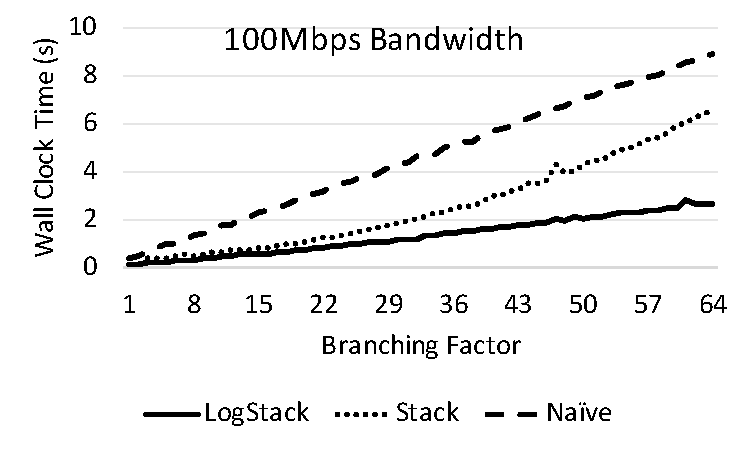
\includegraphics[width=0.4\textwidth]{fig/100mbps}
    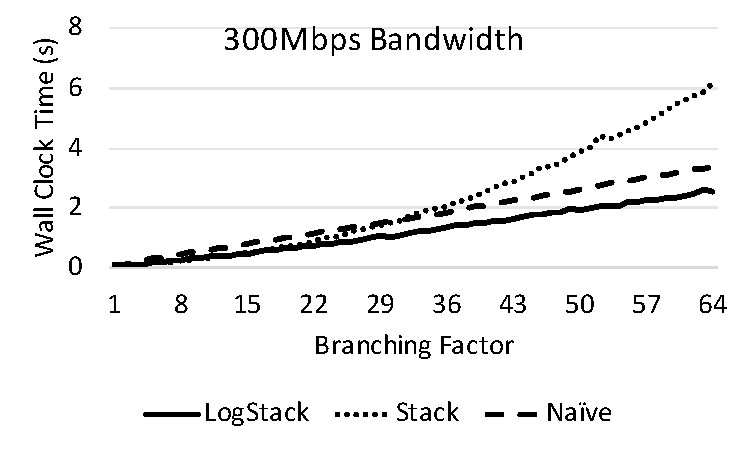
\includegraphics[width=0.4\textwidth]{fig/300mbps}
    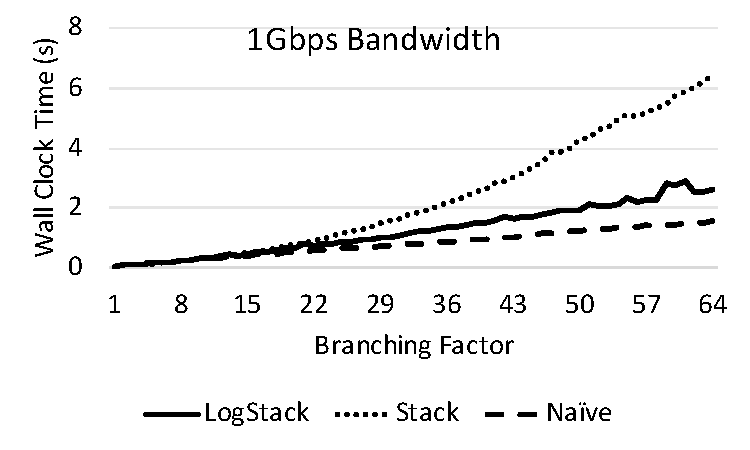
\includegraphics[width=0.4\textwidth]{fig/1gbps}
  	\\
    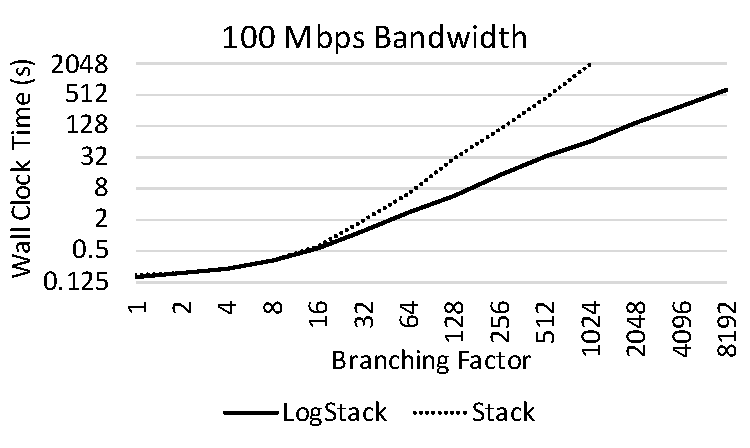
\includegraphics[width=0.4\textwidth]{fig/highbranching}
    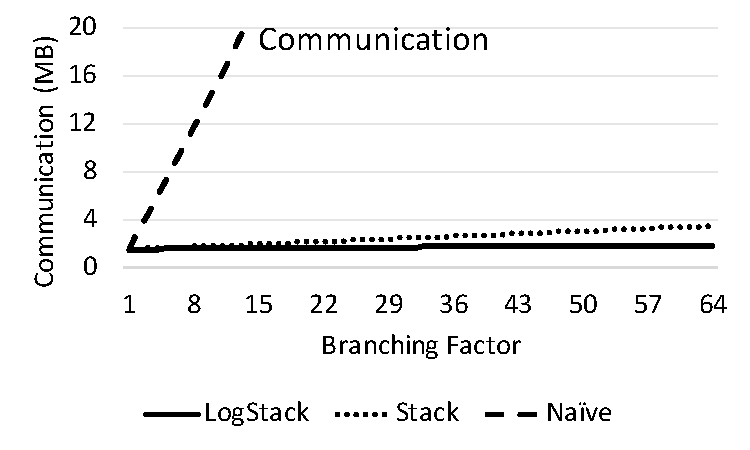
\includegraphics[width=0.4\textwidth]{fig/comm}
    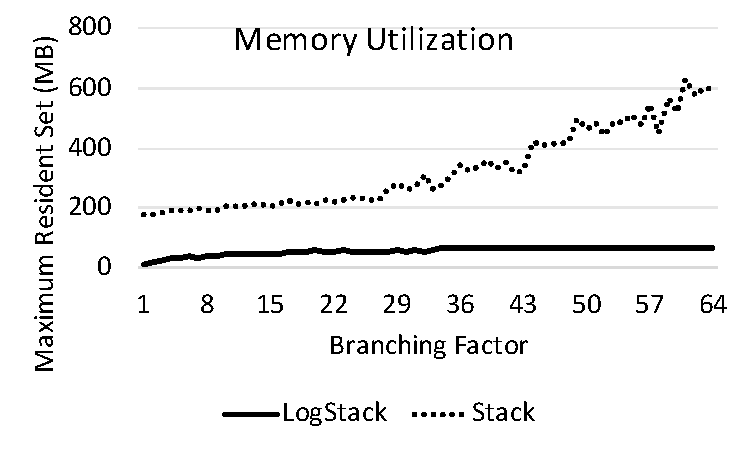
\includegraphics[width=0.4\textwidth]{fig/memutil}
  \end{adjustwidth}
  \caption{%
    Experimental evaluation of \ourschemelong\ as compared to  \HK's
    \stack and to basic half-gates~\cite{EC:ZahRosEva15} (`na\"ive'
    branching).
    We compare in terms of wall-clock time on different simulated network
    bandwidths (top).
    We performed an extended wall-clock time comparison to \stack
    (bottom left).
    Both \ourschemelong\ and \stack\ greatly outperform basic
    half-gates in terms of total bandwidth consumption (bottom
    center), and \ourschemelong\ greatly outperforms \stack\ in terms
    of memory consumption (bottom right).
  }\label{fig:plots}
\end{figure}

We compared our implementation
to implementations of basic half-gates~\cite{EC:ZahRosEva15} and the
\stack SGC of~\HK.
\Cref{fig:plots} plots the results of our experiments.

We consider end-to-end wall-clock time, bandwidth consumption, and memory utilization.
% of 2PC implemented with each of the three schemes and executed with varying number of branches. 
All branches implement the SHA-256 netlist, which has $47726$ AND gates,
$179584$ XOR gates, and $70666$ NOT gates.
A GC for each branch has size $1.45$ MB.
It is, of course, unrealistic that a conditional would have the same
circuit in each branch. However, we choose this benchmark because
SHA-256 has become somewhat of a community standard and because our
goal is only to analyze performance.
%
We ensure our implementation does not cheat: it cannot recognize
that branches are the same and hence cannot shortcut the evaluation.

\paragraph{Total Bandwidth Consumption}  is the easiest metric to analyze.
The communication chart in~\Cref{fig:plots} plots communication
as a function of branching factor.  As expected, \stack's and
\ourschemelong's communication remains almost constant, while half-gates'
grows linearly and immediately dominates.  \ourschemelong is slightly
leaner than \stack because of low-level improvements to
\ourschemelong's demultiplexer. This small improvement should not be counted
as a significant advantage over \stack.

\paragraph{Memory Utilization} was measured as a function of branching
factor.
We compare our scheme to \stack (half-gates memory utilization is
constant, since garblings
can be streamed across the network and immediately discarded).
%
Our chart shows \stack's linear and
\ourschemelong's logarithmic space consumption.
% While \stack uses modest
% space in our experiments, our experiments are on relatively
% small circuits.  For larger branch sizes and more branches, its memory
% consumption may become a bottleneck.  In contrast, our memory
% utilization scales well both with increased branch size and the number
% of branches.
In settings with many branches, improved space consumption
is essential.
For example, we ran \ourschemelong\ on a circuit
with $8192$ SHA-256 branches, a circuit that has $> 385$M
AND gates.  Our peak memory usage was $\sim 100$MB, while \HK
would require more than $12$GB of space to run this experiment.
It would be
infeasible to run this \stack\ experiment on our machine because it
would exhaust our RAM.

\paragraph{Total wall-clock time} to complete an end-to-end 2PC
protocol is our most comprehensive metric.
We plot three charts for 1 to 64
branches (on networks with 100, 300, and 1000 Mbps bandwidth) comparing each of the three approaches.
We also explored more extreme branching factors, running conditionals with
branching factors at every power of $2$ from $2^0$ to $2^{13}$ in the 100Mbps setting.

In the 1Gbps network setting, as expected, na\"ive half-gates leads.
As discussed in~\Cref{sec:whentouse}, two cores (our laptop) indeed
cannot keep up with the available network capacity.  However, doubling
the number of cores would already put us ahead of na\"ive, and any
further computation boost would correspondingly improve
our advantage.  We are about $3\times$ faster than \stack.

In the 300Mbps network setting, we outperform na\"ive.  Because we
range over the same number of branches, we are the same
factor $\approx 3\times$ faster than \stack.

The more typical $100$Mbps setting shows the advantage of SGC.
Both \stack and \ourschemelong handily beat na\"ive.

Finally, we experimented with large branching factors.
\ourschemelong scales well; we ran up to $8192$ branches as it
was sufficient to show a trend.  Due to its logarithmic memory
utilization, \ourschemelong would run on a practically
arbitrary number of branches.  In contrast, \stack exhibited limited
scaling.  We ran up to $1024$ branches with
\stack, enough to show a trend, and after which our experiments
started to take too long.   \ourschemelong ran 2PC for a
$1024$-branch conditional in $\sim 67s$, while \stack took $\sim
2050s$,  $\sim 31\times$ slower than \ourschemelong.




\bibliographystyle{alpha}
\bibliography{bib/bib,bib/abbrev3,bib/crypto,custom}

\newpage

\iffull
{\LARGE \bf \verb+    + Supplementary Material}

\begin{appendix}
\section{Efficiency Proofs}\label{supp:effproofs}

In this section, we prove lemmas regarding the efficiency of
$\gbtree$, $\evcond$, and $\gbcond$.
\Cref{thm:efficiency} follows as a corollary of these lemmas.

\subsubsection{\gbtree\ Efficiency.}

\begin{lemma}\label{lemma:gbtreetime}
  Let $\vec{\cir}$ be a vector of $b$ circuits,
  let $i, j \in \{0, b-1\}$ satisfy $i \leq j$,
  and let $seed \in \{0, 1\}^\kappa$ be an arbitrary string.
  Then $\gbtree(\vec \cir, i, j, seed)$ invokes $\ourscheme.\gGb$ $j - i + 1$ times.
\end{lemma}
\begin{proof}
  Immediate. The procedure only invokes $\ourscheme.\gGb$ at the base case.
\end{proof}
The algorithm garbles each branch only once.
Note that while \Cref{lemma:gbtreetime} (and also
\Cref{lemma:gbtreespace}) holds for all $i, j$, we are
only concerned with it holding for $i, j$ that represent valid nodes
in the binary tree of circuits.


\begin{lemma}\label{lemma:gbtreespace}
  Let $\vec{\cir}$ be a vector of $b$ circuits,
  let $i, j \in \{0, b-1\}$ satisfy $i \leq j$,
  and let $seed \in \{0, 1\}^\kappa$ be a arbitrary string.
  If $\ourscheme.\Gb$ runs in $O(\nmat)$ space,
  then $\gbtree(\vec \cir, i, j, seed)$ runs in $O(\nmat \log (j-i+1))$ space.
\end{lemma}
\begin{proof}
  In the base case, $\gbtree$ invokes $\ourscheme.\gb$. By assumption, this runs
  within our space requirement, and generates a garbling of maximum
  size $\nmat$.
  %
  In the general case, $\gbtree$ recursively invokes itself twice.
  After the first call has finished, we must store the
  intermediate result $M_L$.
  %
  Thus, at each recursive call site, we store a string of size
  $O(\nmat)$.
  Because each recursive call divides the range of considered circuits
  in half, the recursive tree has depth $O(\log(j-i+1))$.
  Hence, the total required storage is $O(\nmat \log(j-i+1))$.
\end{proof}



\subsubsection{\evcond\ Efficiency.}
In terms of time complexity, we start by examining the \emph{concrete}
efficiency on conditionals with $2^k$ branches for some $k$.
%
After, we discuss a generalization to arbitrary numbers of branches.

\begin{lemma}\label{lemma:evcondtime}
  Let $b = 2^k$ for some $k \in \mathbb{N}$.
  Let $\vec{\cir}$ be a vector of $b$ circuits, $\mat$ be a string of
  length $\nmat$, and $\gcirinp$ be a vector of labels of length
  $\inpsize(\conditional(\vec{\cir}))$.
  $\evcond(\vec{\cir}, \mat, \gcirinp)$ calls $\ourscheme.\gGb$ $b \log b$ times
  and calls $ourscheme.\gEv$ $b$ times.
\end{lemma}
\begin{proof}
  First, it is trivial that $\ourscheme.\gEv$ is called $b$ times: the
  procedure is called only at the base case, which is reached once per
  leaf.

  Second, \gbtree\ is called twice in the general case, each on a
  subtree of half of the current branches.
  %
  For example, at the root \gbtree\ is called on every branch, which, by
  \Cref{lemma:gbtreetime}, implies $b$ calls to $\ourscheme.\Gb$.
  Now consider a binary tree whose leaves are the $b$
  branches and whose internal nodes each correspond to
  a recursive invocation of $\evcond'$.
  At every level of the tree, each internal node garbles every
  leaf below it, via \gbtree.
  Hence, every level of the tree entails $b$ calls to $\ourscheme.\Gb$.
  Since the binary tree has $\log b$ levels, there are $b
  \log b$ total calls to $\ourscheme.\Gb$.
\end{proof}

By essentially exactly the same argument, one can prove the following
lemma for arbitrary numbers of branches:
\begin{lemma}\label{lemma:evcondtime-general}
  Let $\vec{\cir}$ be a vector of $b$ circuits, $\mat$ be a string of
  length $\nmat$, and $\gcirinp$ be a vector of labels of length
  $\inpsize(\conditional(\vec{\cir}))$.
  $\evcond(\vec{\cir}, \mat, \gcirinp)$ calls $\ourscheme.\gGb$ $O(b \log b)$ times
  and calls $\ourscheme.\gEv$ $b$ times.
\end{lemma}

The following lemma formalizes \evcond's logarithmic space complexity:
\begin{lemma}\label{lemma:evcondspace}
  Let $\vec{\cir}$ be a vector of $b$ circuits, $\mat$ be a string of
  length $\nmat$, and $\gcirinp$ be a vector of labels of length
  $\inpsize(\conditional(\vec{\cir}))$.
  $\evcond(\vec{\cir}, \mat, \gcirinp)$ runs in $O(\nmat \log b)$ space.
\end{lemma}
\begin{proof}
  Trivial, since no material is stored at recursive call sites.
  Thus the space complexity is inherited from
  \gbtree~(\Cref{lemma:gbtreespace}).
\end{proof}



\subsubsection{\gbcond\ Efficiency.}
As with \evcond, we start with a concrete claim
regarding conditionals with branching factors that are powers of two:

\begin{lemma}\label{lemma:gbcondtime}
  Let $b = 2^k$ for $k \in \mathbb{N}$.
  Let $\vec{\cir}$ be a vector of $b$ circuits and $S \in \{0,
  1\}^\kappa$ be a string.
  $\gbcond(\vec{\cir}, S)$ calls $\ourscheme.\gGb$ $\frac{3}{2}b \log b + b$ times and calls
  $\ourscheme.\gEv$ $b\log b$ times.
\end{lemma}
\begin{proof}
  First, we handle the $b$ $\ourscheme.\gGb$ calls. These $b$ calls arise from the
  top-level call to $\gbtree$ in $\gbcond$.
  The remaining $\frac{3}{2} b \log b$ calls come from
  \computegarbage.
  %
  Our argument is similar to that of \Cref{lemma:evcondtime}:
  at each level of the binary tree, $\computegarbage$ calls
  $\ourscheme.\gGb$ $\frac{3}{2}b$ times (via each node's three calls to \gbtree\
  on half of the node's ancestors).
  Since there are $\log b$ levels in the tree, $\computegarbage$ calls
  $\ourscheme.\gGb$ a total of $\frac{3}{2}b \log b$ times.

  All calls to $\ourscheme.\gEv$ arise from $\computegarbage$.
  In particular, $\ourscheme.\gEv$ calls occur in the base case (reached once per
  branch).
  Each branch is evaluated $\log b$ times: once per appropriate
  combination of garbage material. Since each leaf has $\log b$
  sibling roots, the vector $\vec{\mat}'$ has $\log b$ members.
  %
  Hence, we invoke $\ourscheme.\gEv$ a total of $b \log b$ times.
\end{proof}

By essentially the same argument, the following claims holds
for conditionals with arbitrary branching factors:
\begin{lemma}\label{lemma:gbcondtime-general}
  Let $\vec{\cir}$ be a vector of $b$ circuits and $S \in \{0,
  1\}^\kappa$ be a string.
  $\gbcond(\vec{\cir}, S)$ calls \gGb\ $O(b \log b)$ times and calls
  $\gEv$ $O(b\log b)$ times.
\end{lemma}

Finally, \gbcond\ runs in logarithmic space:
\begin{lemma}\label{lemma:gbcondspace}
  Let $\vec{\cir}$ be a vector of $b$ circuits and $S \in \{0, 1\}^\kappa$ be a string.
  If $\gGb$ runs in $O(\nmat)$ space, then
  $\gbcond(\vec{\cir}, S)$ runs in $O(\nmat \log b)$ space.
\end{lemma}
\begin{proof}
  Like $\evcond$, \gbcond\ consumes space due to calls to
  $\gbtree$. However, by \Cref{lemma:gbtreespace}, each of these calls
  runs in $O(\nmat \log b)$ space.
  %
  Additionally, \computegarbage\ maintains a vector of material
  $\vec{\mat}'$.
  However, this vector's size is bounded by the depth of the tree: we
  concatenate one material to the vector at each recursive call
  site.
  Hence, $\vec{\mat}'$ holds $O(\log b)$ elements and hence has
  $O(\nmat \log b)$ size.
\end{proof}

\section{Correctness/Security Proofs}\label{supp:proofs}

% \begin{theorem}\label{theorem:correctness}
%   If \underscheme\ is correct, then \ourschemelong\ is correct.
% \end{theorem}
The following proves \Cref{theorem:correctness}, i.e. \ourschemelong\
is correct:
\begin{proof}
  By induction on structure of $\cir$.
  \begin{itemize}
    \item Suppose \cir\ is a netlist. Then since \ourschemelong\ delegates
      to the correct scheme \underscheme, \ourschemelong\ is trivially
      correct.
    \item Suppose \cir\ is a sequence $\sequential(\cir_0, \cir_1)$.
      By induction, both $\cir_0$ and $\cir_1$ correctly propagate
      input labels to output labels.
      Thus, to finish the proof, we must show that we appropriately
      translate output labels from $\cir_0$ to $\cir_1$. But this is
      the role of the translator component, which is trivially correct
      as it is implemented by garbled rows~\HK.
    \item Suppose \cir\ is a conditional $\conditional(\vec \cir)$.
      Consider an arbitrary execution where the branch $\cir_\act$ is
      active.
      %
      By definition, the first $\lceil \log |\vec \cir| \rceil$ input
      labels to \gEv\ are an encoding of \act.
      %
      Recall that \gGb\ constructs the material $M = \bigoplus_i
      \gcir_i$: this is the material available to \gEv.
      %
      Due to the correctness of \gadget, \gEv\ computes the correct
      sibling roots of $\cir_A$. Thus, \evcond\ reconstructs the correct
      garblings $\gcir_{i \neq A}$, XORs these with $M$, and hence
      extracts $\gcir_A$.

      Now, it remains to show two points.
      First, we must show that the inputs are correctly fed to
      $\cir_A$. The second is to show that the garbage values from all
      branches $\cir_{i \neq A}$ are collected.
      %
      The first point is handled by the demultiplexer.
      %
      The demultiplexer implements via garbled rows simple logic: the
      correct input is forwarded to $\cir_A$, and garbage labels (that
      are independent of the input) is forwarded to all other circuits
      $\cir_{i \neq A}$.
      %
      The second point is handled by the multiplexer, generated by the
      emulation of all possible garbage branch evaluations.
      %
      We refer the reader to \Cref{sec:techOverview} for an extensive
      discussion of how this emulation is achieved.
      %
      In short, we carefully arrange \gadget\ such that there are
      only $\lceil \log |\vec \cir| \rceil$ garbage evaluations
      possible per branch.
      %
      Because the number of garbage evaluations is small, it is easy
      for \gGb\ to compute all of these cases itself.
      %
      With all possible garbage output labels available, garbage
      collection becomes the straightforward implementation of garbled
      rows.
      %In particular, consider a single corresponding output wire
      %from each branch.
      %%
      %The multiplexer first XORs together these labels.
      %Now, it uses \act\ to construct garbled rows that hold all
      %possible garbage values for this wire.
      %Thus, depending on \act, \gEv\ will decrypt exactly the garbage
      %values that were XORed into the overall sum.
      %%
      %XORing these with the overall sum leaves only the valid output.
  \end{itemize}
  \ourschemelong\ is correct.
\end{proof}

The following proves \Cref{thm:strongstack}, i.e. \ourschemelong\ is
strongly stackable.
\begin{proof}
  By induction on the structure of \cir.
  We say `$x$ looks random' to denote that $x$ is indistinguishable from a uniform string of the same length.
  \begin{itemize}
    \item Suppose \cir\ is a netlist.
      Then $\ourschemelong$ delegates to \underscheme,
      which is assumed to be strongly stackable.
    \item Suppose \cir\ is a sequence $\sequential(\cir_0, \cir_1)$.
      By induction,
      both $\cir_0$ and $\cir_1$ are strongly stackable.
      We demonstrate that the intervening translation
      gadget preserves strong stackability.
      %
      Consider a subcomponent of the translator that translates one wire.
      %
      This subcomponent is implemented as an encrypted truth table with two ciphertexts of material.
      %
      Each row is the XOR of an input label with the
      output
      of a PRF keyed at the $\lkey$ of a label specified by the
      decoding string $d_0$ of $\cir_0$.
      Since $\cir_0$ is strongly stackable, this key looks random.
      Hence, the output of the PRF looks random.
      Furthermore, correctly decrypting one row yields an
      input label for $\cir_1$ which, by induction, looks random.
      %
      Therefore, the ciphertexts constructed by $\gbtranslate$
      look random, so the translation gadget preserves strong stackability.
    \item Suppose \cir\ is a conditional $\conditional(\vec \cir)$.
      By induction, each branch $\cir_i \in \vec \cir$ is strongly
      stackable.
      Hence, the material from each branch looks random, and so the
      XOR stacking of all materials looks random as well.
      %
      It remains to show that \gadget, the demultiplexer, and the multiplexer
      preserve strong stackability.
      Like the translator (see discussion of sequences
      above), these gadgets are constructed using a PRF, and hence
      their material looks random.
      %
      An additional important detail is that \gadget\ outputs good
      seeds only for the sibling subroots of the active branch \aid.
      Recall that the good seed for each node in the binary
      tree is derived from its parent's seed, so it may seem there is
      a possibility that \E can check if seeds are related to one
      another.
      %
      However, because \gadget\ gives only good seeds corresponding to
      sibling roots of a fixed (active) branch, all seeds seen by \E\ are
      unrelated.
      %
      Finally, \E\ reconstructs, via seeds, the good garbling of each
      circuit $\cir_{i\neq\aid}$. Thus, she sees the input encoding
      for each branch $\cir_{i\neq\aid}$.
      %
      Thus, it may seem that \E\ can compare input encodings of
      each branch with that branch's input labels.
      %
      However, the demultiplexer computes, based on \aid, garbage inputs
      unrelated to each of these encodings, and hence the outputs of
      the demultiplexer and the garblings of each branch are
      unrelated.
  \end{itemize}
  Finally,
  all encodings directly handled our gadgets are either given to us by
  \underscheme, our are uniformly drawn (with appropriate color bits), and
  hence we satisfy properties 2 through 4.
  \ourschemelong\ is strongly stackable.
\end{proof}

The following proves \Cref{thm:authenticity}, i.e. \ourschemelong\ is
authentic.
\begin{proof}
  By induction on the structure of the circuit $\cir$.
  In each case, we proceed backwards across the components of $\cir$ (i.e. from outputs to inputs), at
  each step showing that $\adv$ cannot obtain valid labels
  except by running the previous components of the circuit.
  \begin{itemize}
    \item Suppose $\cir$ is a netlist. \ourschemelong delegates to
      \underscheme which is assumed authentic.
    \item Suppose $\cir$ is a sequence $\sequential(\cir_0, \cir_1)$.
      By induction, \adv\ cannot obtain valid
      output from $\cir_1$ except by running $\gEv$.
      %
      Furthermore, the intervening translator gadget is authentic: it
      is constructed by masking the translator output label with a PRF call
      keyed at the respective translator input label.
      %
      Thus, \adv\ cannot compute a translator output label without providing
      a corresponding input label from the output of $\cir_0$.
      %
      Finally, $\cir_0$ inductively preserves authenticity.
      %
      Thus, the sequence is authentic.
    \item Suppose $\cir$ is a conditional $\conditional(\vec{\cir})$.
      %
      First, we examine the mux. Using the same argument as for the
      translator (the mux is built using a PRF), valid output cannot be obtained except by running $\evmux$ on valid inputs.

      Inputs to the mux component are constructed by evaluating
      each branch $\cir_i$.
      %
      By induction $\cir_\aid$ is authentic, and so $\adv$ cannot
      obtain output labels from the active circuit without providing
      corresponding input labels.
      %
      Note, each circuit $\cir_{i \neq \aid}$ is not supported by our
      inductive argument, since we operate on these circuits with
      garbage labels and material.
      %
      However, because the output of the multiplexer is masked by a
      PRF call on outputs from \emph{each} branch, it suffices that
      $\cir_\aid$ is authentic.

      Finally, consider the demultiplexer and \gadget. $\adv$ cannot construct valid
      input to $\cir_\aid$ except by running these components: they
      are built using a PRF.
      %
      Thus, the overall conditional is authentic.
  \end{itemize}
  \ourscheme is authentic.
\end{proof}


The following proves \Cref{thm:privacy}, i.e. \ourschemelong\ is
private.
\begin{proof}
  By induction on the structure of $\cir$.
  \begin{itemize}
    \item Suppose \cir\ is a netlist. \ourschemelong\ delegates to
      \underscheme\ which is assumed private.
    \item Suppose \cir\ is a sequence $\sequential(\cir_0, \cir_1)$.
      Note that the garbling of $\cir_0$ is independent of
      $\cir_1$, and so the garbling of $\cir_0$ cannot give any extra information when combined
      with $d$ from $\cir_1$.
      %
      While the translator gadget is not independent of the garbling
      of $\cir_1$ (its garbled rows include labels from the input
      encoding of $\cir_1$), the information related to $\cir_1$ is
      masked by secure evaluation of a PRF.
      %
      Furthermore, because $\cir_0$ is authentic, there is no feasible
      way for \adv\ to compute any input to the translator which is
      not computed by evaluating $\cir_0$ on a given input.
      % way for \adv\ to compute input labels to the translator that cannot be
      % simulated.
      %
      Thus, the following simulator suffices:
      \begin{align*}
        &\simulator_{prv}(1^\kappa, \sequential(\cir_0, \cir_1), \cirout):\\
        &~~(\mat_0, \gcirinp_0) \gets \simulator_{obv}(1^\kappa, \cir_0)\\
        &~~\gcirout \gets \gEv(\cir_0, \mat_0, \gcirinp_0)\\
        &~~(\mat_1, \gcirinp_1, d) \gets \simulator_{prv}(1^\kappa, \cir_1, \cirout)\\
        &~~\mat_{tr} \gets \simulator_{tr}(\gcirout, \gcirinp_1)\\
        &~~\creturn~(\mat_0 \mid \mat_{tr} \mid \mat_1, \gcirinp_0, d)
      \end{align*}
      Where $\simulator_{tr}$ simulates a translator
      mapping the encoded output $\gcirout$ to the encoded input
      $\gcirinp_1$ (other rows that do not involve the labels in
      $\gcirinp_1$ are simulated by uniformly sampling strings).
    \item Suppose \cir\ is a conditional $\conditional(\vec \cir)$.
      % Note first that the garbling of each branch is independent from
      % the multiplexer, except that output labels from each branch are
      % used as PRF keys.
      In this case, the privacy simulator (1) garbles the conditional
      using a uniform seed, (2) encodes an arbitrary input (say, the
      all 0s input), and (3) evaluates the conditional.
      Now, the simulator holds material $\mat$, an encoded input
      $\gcirinp$, an output decoding $d$, and an encoded output
      $\gcirout$.
      The simulator conditionally swaps the labels in $d$ based on the
      output $\cirout$ such that $\gDe(d, \gcirout) = \cirout$ and
      outputs $(\mat, \gcirinp, d)$.
      Note, labels in $d$ are uniformly chosen by a call to
      $\genprojection$.
      Furthermore, the active branch $\cir_\aid$ is authentic, and
      hence there is no feasible way for \adv\ to compute any input to
      the multiplexer which is
      not computed by evaluating $\cir_\aid$ on a given input.
      %
      Thus, undecryptable multiplexer rows are securely simulated by
      random bits.
      % Thus, these labels are computationally indistinguishable from
      % uniform strings.
      $(\mat, \gcirinp, d)$ is indistinguishable from the real view.
  \end{itemize}
  \ourschemelong\ is private.
\end{proof}

\section{Universal Circuits}
We use cryptographic techniques to reduce the cost of conditionals.
Our focus is the reduction of communication to that corresponding to
the longest branch (SGC), while keeping the computational cost low.
A related direction attempts to instead reduce such 2PC cost by
choosing alternate Boolean circuit representations.  Universal
circuits (UCs) can be \emph{programmed} to implement any circuit in
the entire universe of circuits of a given size
$n$~\cite{STOC:Valiant76}.  Researchers continue to search for smaller
UC constructions; recent work achieves size $\approx 4.5 |C| \log
|C|$~\cite{EPRINT:LipMohSad16,EC:KisSch16,AC:GunKisSch17,EPRINT:ZYZL19,EPRINT:AGKS19}.
%
UCs implement conditionals by programming the UC to be the taken
branch.  When the GC generator knows the evaluated branch, the cost of
UC programming is free as the generator directly programs the UC;
otherwise programming can be achieved by transferring the right
garbled table via OT, as, e.g., proposed in~\cite{AC:KenKolWil17}.
This causes further $\approx 5\times$ overhead.

There are several shortcomings of this approach.  Firstly,  $5\cdot
4.5 |C| \log |C|$ %(and even $4.5 |C| \log |C|$ cost of the free
programming case) is a significant {\em communication} cost, compared
to our cost $|C|$.  For example, even for branches with only $2^{10}$
gates, the UC is $5 \cdot 4.5 \cdot 10 = 225$ times larger than a
single branch.  For typical conditionals it is often much cheaper to
separately encrypt and send each branch.  Further, general branching
implementation for GC proposed in~\cite{AC:KenKolWil17} is not
constant-round, and requires a round of communiction for every
sequential conditional.


Focusing specifically on branching,~\cite{AC:KenKolWil17} proposed a
generalization of UCs called \emph{set} universal circuits ($\cal
S$-UCs).  An $\cal S$-UC implements a fixed set of circuits $\cal S$
rather than an entire size-$n$ universe.  \cite{AC:KenKolWil17}
focuses on the special case where $|\cal S|$ is small, capturing the
case where $\cal S$ is a set of conditional branches.  Their approach
applies heuristics to embed $\cal S$ into one programmable circuit.
\cite{AC:KenKolWil17} reports the performance of this heuristic for
specific sets of circuits, achieving up to $6\times$ GC size reduction
for $32$ branches.  However, some sets did not improve over their
original representations.  Our work always achieves size reduction to
that of the single (largest) branch. In the~\cite{AC:KenKolWil17}
example, we achieve up to $32\times$ GC size reduction for $32$
branches and requires no per-gate overhead, which is significant
in~\cite{AC:KenKolWil17} (about $22$ garbled rows per gate).  


\end{appendix}

\else

% these references only appear in the supplementary material: cite
% them anyway


\fi

\end{document}
